\chapter{Heat Transfer Modelling and Simulation}
\label{Cap:Thermal}

It is desirable to theoretically analyse a new solar energy system, such as any given system, before the prototype fabrication (\cite{Tchinda2008}). A thermal model for the simulation of a solar air heater is an important tool for predicting its long-term performance under different weather conditions (\cite{Shams2013}). Therefore, this chapter aims to: 

\begin{itemize}[topsep=5pt,partopsep=0pt] \itemsep0pt
	\item develop a heat transfer model to simulate the thermal performance of the proposed solar air heater when in operation;
	\item validate the model against experimental data from the tests described in Chapter \ref{Cap:Exp};
	\item simulate the model composed of multiple collectors connected;
	\item simulate a barley drying operation using the results from the thermal modelling.
\end{itemize}

Consequently, the specific objectives of this chapter are to:

\begin{itemize}[topsep=5pt,partopsep=0pt] \itemsep0pt
	\item simulate the collector under different solar radiation levels and airflow rates;
	\item estimate outlet airflow temperatures;
	\item evaluate the system's thermal efficiency;
	\item determine useful energy delivered to the airflow;
	\item calculate the useful energy and outlet temperatures for connected collectors;
	\item estimate how much energy the solar air heating system (SAHS) can provide to a barley dryer.
\end{itemize}

The model will be employed to gain insight into and understand the interactions between system inputs and outputs, as shown in Figure \ref{block_diagram}. The model algorithm implemented for simulation was created to predict behaviour under transient state conditions. 

\Figure[scale=0.50,placement=!ht,label={block_diagram},caption={Block diagram of the heat transfer model.},shortcaption={Block diagram of the heat transfer model}]{figs/block_diagram.eps}

\section{Solar air heating collector's heat transfer modelling}

The first step for modelling the solar air heating system is establishing the collector's components to be modelled for simulation. In this cas,e there are three: the first one is the absorber surface, the second one is the glazing cover, and the last one is the airflow inside the collector. The next step is to state assumptions in order to simplify the model, which are listed as follows:

\begin{itemize}
	\item Solar radiation is incident uniformly over the components' surfaces;
	\item Absorber and glazing temperatures are uniform;
	\item Thermal and physical properties of the components are independent of temperature;
	\item Heat transfer at the reflectors and wooden cavity and conduction losses are neglected;
	\item The airflow rate is uniform through all the absorber holes;
\end{itemize}

The following step of the modelling depicts how the energy balance in the components is evaluated according to the following statements:

\begin{equation*}
\left( \begin{array}{l}
{\rm{\ \ \ \ \ \ Rate \ of}}\\
{\rm{\ internal \ energy }}\\
{\rm{\ in \ the \ absorber}}
\end{array} \right) = \left( \begin{array}{l}
{\rm{Absorbed \ solar}}\\
{\rm{\ \ radiation \ in}}\\
{\rm{\ \ the \ absorber}}
\end{array} \right) - \left( \begin{array}{l}
{\rm{\ \ Heat \ losses}}\\
{\rm{from \ absorber}}
\end{array} \right) - \left( \begin{array}{l}
{\rm{Useful \ heat}}\\
{\rm{ rate \ to \ airflow}}
\end{array} \right)
\label{text_equation_ABS}
\end{equation*}
\vspace*{-0.10cm}
\begin{equation*}
\left( \begin{array}{l}
{\rm{\ \ \ \ \ \ Rate \ of}}\\
{\rm{\ internal \ energy }}\\
{\rm{\ in \ the \ glazing}}
\end{array} \right) = \left( \begin{array}{l}
{\rm{Absorbed \ solar}}\\
{\rm{\ \ radiation \ in}}\\
{\rm{\ \ the \ glazing}}
\end{array} \right) + \left( \begin{array}{l}
{\rm{\ \ Heat \ losses}}\\
{\rm{from \ absorber}}
\end{array} \right) - \left( \begin{array}{l}
{\rm{Heat \ losses}}\\
{\rm{from \ glazing}}
\end{array} \right)
\label{text_equation_GLAZ}
\end{equation*}
\vspace*{-0.10cm}
\begin{equation*}
	\left( \begin{array}{l}
		{\rm{\ \ \ \ \ \ Rate \ of}}\\
		{\rm{\ useful \ energy }}\\
		{\rm{\ in \ the \ airflow}}
	\end{array} \right) = \left( \begin{array}{l}
		{\rm{Convective \ heat}}\\
		{\rm{\ transfer \ from \ the \ }}\\
		{\rm{\ \ absorber \ plate}}
	\end{array} \right) - \left( \begin{array}{l}
		{\rm{\ \ Heat \ losses}}\\
		{\rm{from \ airflow \ }} \\
		{\rm{to \ the \ glazing \ }}
	\end{array} \right) 
	\label{text_equation_air}
\end{equation*}

%\noindent where the heat losses are convective and radiative. %Translating the previous expressions into variables, Eqs. (\ref{EBabsorber1}) and (\ref{EBglazing1}) are obtained:

%\begin{equation}
%\mathrm{\frac{{d{U_{abs}}}}{{dt}} = {S_{abs}} - {Q_{\!_{L,1}}} - {Q_u}}
%\label{EBabsorber1}
%\end{equation}
%\vspace*{-0.5cm}
%\begin{equation}
%\mathrm{\frac{{d{U_{glaz}}}}{{dt}} = {S_{glaz}} + {Q_{\!_{L,1}}} - {Q_{\!_{L,2}}}}
%\label{EBglazing1}
%\end{equation}

\noindent where the heat losses are convective and radiative. In order to visualise how these heat rates are placed, Figure \ref{thermal_network} presents the collector's thermal network as an analogy to an electric circuit, where the absorber, glazing and air inside the collector are nodes. The energy input here is the total solar radiation $\rm{I_{\!_{T}}}$, and mathematical expressions above each resistor were used to calculate the thermal resistances.

\Figure[scale=0.75,placement=!ht,label={thermal_network},caption={Thermal network to illustrate heat flows in the air heater, where the subscripts C and R refer to convection and radiation, respectively.}, shortcaption={Thermal network to illustrate heat flows in the air heater.}]{figs/resistances.png}

From the absorber node, the circuit path to the right is the heat transfer path to the airflow (upper path) and radiative (lower path) heat losses. At the upper path, there is also the convective resistance from the airflow to the glazing, indicating convective loss inside the collector. Similarly, there are losses from glazing to the ambient, as indicated by the thermal resistances to the right of its node. These heat transfer types will be addressed later. Applying the concept of heat loss rate as the ratio of temperature difference to the corresponding thermal resistance:

\vspace{-0.75cm}
\begin{equation}
\mathrm{{M_{abs}}{C_{p,abs}}\frac{{d{T_{abs}}}}{{dt}} = {S_{abs}} - \left( {\frac{{{T_{abs}} - {T_{air}}}}{R_{\!_{HX}}} + \frac{{{T_{abs}} - {T_{glaz}}}}{R_{\!_{R1}}}} \right) }
\label{eqabsorber1}
\end{equation}
\vspace*{-0.25cm}
\begin{equation}
\mathrm{{M_{glaz}}{C_{p,glaz}}\frac{{d{T_{glaz}}}}{{dt}} = {S_{glaz}} + \left( {\frac{{{T_{air}} - {T_{glaz}}}}{R_{\!_{C1}}} + \frac{{{T_{abs}} - {T_{glaz}}}}{R_{\!_{R1}}}} \right) - \frac{{{T_{glaz}} - {T_{amb}}}}{{{\displaystyle{\left( {\frac{1}{{{R_{\!_{C2}}}}} + \frac{1}{{{R_{\!_{R2}}}}}} \right)}^{-1}}}}}
\label{eqglazing1}
\end{equation}
\vspace*{-0.25cm}
\begin{equation}
	\mathrm{G_{air}A_{abs}C_{p,air}\frac{dT_{air}}{dt} = \frac{(T_{abs} - T_{air})}{R_{\!_{HX}}} - \frac{(T_{air} - T_{glaz})}{R_{\!_{C1}}}}
	\label{EBair1}
\end{equation}

Substituting the thermal resistances by the mathematical expressions properly and isolating the derivative terms, Eqs. (\ref{EBabsorber2}), Eq. (\ref{EBglazing2}) and Eq. (\ref{EBair2}) are obtained.

\vspace{-0.75cm}
\begin{equation}
\mathrm{\frac{{d{T_{abs}}}}{{dt}} = \frac{1}{{M _{abs}}{C_{p,abs}}} \left[S_{abs} - {h_{\!_{R1}}}{A_{abs}}({T_{abs} - T_{glaz}}) - {h_{\!_{HX}}A_{abs}(T_{abs} - T_{air})} \right]} 
\label{EBabsorber2}
\end{equation}
\vspace*{-0.25cm}
\begin{equation}
\mathrm{\frac{{d{T_{glaz}}}}{{dt}} = \frac{1}{{{M_{glaz}}{C_{p,glaz}}}}}\left[ \begin{array}{l}
\mathrm{{S_{glaz}} + {h_{\!_{R1}}}{A_{abs}}( {{T_{abs}} - {T_{glaz}}} ) + {h_{\!_{C1}}}{A_{abs}}( {{T_{air}} - {T_{glaz}}} )}\\
\mathrm{- ( {{h_{\!_{R2}}} + {h_{\!_{C2}}}} ){A_{glaz}}( {{T_{glaz}} - {T_{amb}}} )}
\end{array} \right]
\label{EBglazing2}
\end{equation}
\vspace*{-0.25cm}
\begin{equation}
	\mathrm{G_{air}A_{abs}C_{p,air}\frac{dT_{air}}{dt} = h_{\!_{HX}}A_{abs}(T_{abs} - T_{air}) - h_{\!_{C1}}A_{abs}(T_{air} - T_{glaz})       }
	\label{EBair2}
\end{equation}

%Lastly, the thermal efficiency, which is the ratio of useful heat rate to the incoming total solar radiation on the aperture, is calculated by Eq. (\ref{ThermalEf}). Such efficiency can be evaluated either instantaneously or as an average over a certain period of time (\cite{Goswami2015}).
%
%\begin{equation}
%\mathrm{\mathlarger{\eta}_{\mathrm{th}} = \frac{Q_u}{I_{\!_T}A_{apt}}}
%\label{ThermalEf}
%\end{equation}

The next subsections describe how the absorbed solar radiation terms, convective and radiative heat transfer coefficients, useful energy rate and outlet air temperature from the thermal model were determined.

\subsection{Absorbed solar radiation terms}

%However, it is not possible to measure the amount of $\rm{G_{\!_{T}}}$ to be absorbed in the elements. Hence, it is necessary to estimate how much of the total solar radiation is absorbed by each element.

%The incident solar radiation on the solar collector's aperture undergoes optical losses on glazing cover and reflectors before it reaches the absorber surface. The optical loss on the glazing surface depends on the incident angle which varies over time of day and the absorption property of the glazing material. The optical efficiency varies based on the proportion of the beam and diffuse radiation for a particular time of the day.

%The total solar radiation ($\rm{I_{\!_{T}}}$) incident on the concentrator's aperture is the sum of the beam ($\rm{I_{\!_{B}}}$) and diffuse ($\rm{I_{\!_{D}}}$) components. However, since only part of the diffuse radiation is exploitable by concentrators, the factor $\xi$ must be defined, as being the fraction of total solar radiation accepted. Assuming that the diffuse distribution is isotropic, this factor can be estimated as (\cite{Prapas1987}):
%
%\begin{equation}
%\mathrm{\xi  = \frac{\displaystyle {\left( {{I_{\!_B}} + \frac{{{I_{\!_D}}}}{C}} \right)}}{{{I_{\!_T}}}}}
%\label{IC}
%\end{equation} 
%
%\noindent and therefore the incoming solar radiation available to reach the absorber surface is assumed to be $\rm{I_{\!_T}\xi}$. 
The portion of total solar radiation undergoes optical losses before it reaches the absorber -- expressed in terms of ${\eta_{\!_{0}}}$ and previously discussed in Chapters \ref{Cap:Lit} and \ref{Cap:Opt}. Hence, $\rm{S_{abs}}$ is given by Eq. (\ref{Sabs}).
%In order to estimate $\rm{S_{abs}}$, it is necessary to regard that the portion of incoming solar radiation goes through optical losses -- expressed in terms of ${\eta_{\!_{0}}}$ and previously discussed in Chapter \ref{Cap:Opt}. Therefore, $\rm{S_{abs}}$ is given by Eq. (\ref{Sabs}).

\vspace{-0.75cm}
\begin{equation}
\mathrm{{S_{abs}} = I_{\!_{T}}\Gamma A_{apt}\mathlarger{{\eta_{\!_{0}}}}}
\label{Sabs}
\end{equation}

The absorbed solar radiation by the glazing, which is based on the capacity of this component to retain the incoming radiation incident on the aperture, can be expressed as:

\vspace{-0.75cm}
\begin{equation}
\mathrm{{S_{glaz}} = I_{\!_{T}}A_{apt}{\mathlarger{\alpha}_{\mathrm{glaz}}}}
\label{Sglaz}
\end{equation}

\noindent where the glazing absorptivity $\alpha_{\rm{glaz}}$ was also estimated in Chapter \ref{Cap:Opt}.

\subsection{Radiative heat transfer coefficients}

The radiative heat transfer coefficient from the absorber to the glazing $\rm{h_{\!_{R1}}}$ can be evaluated by Eq. (\ref{hr1}):

\vspace{-0.75cm}
\begin{equation}
\mathrm{{h_{\!_{R1}}} = {\varepsilon _{eff}}\sigma \left( {T_{abs}^2 + T_{glaz}^2} \right)\left( {{T_{abs}} + {T_{glaz}}} \right)}
\label{hr1}
\end{equation}

\noindent where $\rm{\varepsilon_{eff}}$ is the effective emissivity, a radiative property developed by \citet{Rabl1976} for a CPC comprised of specular reflectors. Although the solar air heater to be modelled here is not a simple CPC, such methodology of assessing $\rm{h_{\!_{R1}}}$ was used, given the similarity of both geometries. The calculation of $\rm{\varepsilon_{eff}}$ considers the radiative properties of the absorber, reflector and glazing, such as emissivity and reflectivity, and the concentrator's geometric concentration ratio. 
%Given the assumption os constant properties of the elements defined earlier, this effective emissivity assumes a constant value.

The radiative heat transfer coefficient from the glazing to the ambient $\rm{h_{\!_{R2}}}$ was evaluated by Eq. (\ref{hr2}):

\vspace{-0.75cm}
\begin{equation}
\mathrm{{h_{\!_{R2}}} = {\varepsilon _{glaz}}\sigma \left( {T_{glaz}^2 + T_{amb}^2} \right)\left( {{T_{glaz}} + {T_{amb}}} \right)}
\label{hr2}
\end{equation}

\noindent where the glazing is considered to emit radiation to the ambient only, which absorbs all the emitted energy from that, thus acting as a blackbody (\cite{Duffie2013}).

\subsection{Convective heat transfer coefficients}

In order to calculate the heat transfer coefficient from the airflow to the glazing $\rm{h_{\!_{C1}}}$, it is assumed that the airflow circulating within the collector loses part of its thermal energy to the glazing by convection. Therefore, the estimation of $\rm{h_{\!_{C1}}}$ is given by Eq. (\ref{hc1}) (\cite{Zheng2016}):

\vspace{-0.75cm}
\begin{equation}
\mathrm{{h_{\!_{C1}}} = \frac{k_{air}}{L_{col}}{Nu_{\!_{C1}}} = \frac{{{k_{air}}}}{{{L_{col}}}}\left( {0.664{\rm{Re}}_{\!_{C1}}^{1/2}{\rm{Pr}}^{1/3}} \right)}
\label{hc1}
\end{equation}

\noindent where it is assumed that the air thermal properties are evaluated at the average between $\rm{T_{abs}}$ and $\rm{T_{in}}$; the Reynolds number based on the air velocity at the inlet ($\rm{v_{in}}$) is:

\vspace{-0.75cm}
\begin{equation}
\mathrm{{{\mathop{\rm Re}\nolimits}_{\!_{C1}}} = \frac{{{v_{in}}{L_{col}}}}{{{\mathlarger{\nu}_{air}}}}}
\label{Rec1}
\end{equation}

In order to calculate the heat transfer coefficient from glazing to ambient $\rm{h_{\!_{C2}}}$, it is assumed that the convection loss is forced by the wind. Therefore, the estimation of it is given by Eq. (\ref{wind}) (\cite{Tchinda2008}):

\vspace{-0.75cm}
\begin{equation}
	\mathrm{h_{\!_{C2}} = 2.8 + 3v_w}
	\label{wind}
\end{equation}

%\subsection{Useful energy rate and outlet air temperature}

%The useful heat rate transferred to the airflow is determined by Eq. (\ref{usefulenergy}):
%
%\begin{equation}
%\mathrm{{Q_u} = {G_{air}}{A_{abs}}{C_{p,air}}({T_{out}} - {T_{in}})}
%\label{usefulenergy}
%\end{equation}

%The useful energy rate was given in Eq. (\ref{usefulenergy}). It should be noted that the outlet air temperature is unknown in the modelling. Therefore, understanding heat transfer from the absorber to the airflow becomes necessary to estimate $\rm{T_{out}}$. To do so, another way of assessing $\rm{Q_u}$ is by using fundamentals of heat exchange (\cite{Incropera2006}), which is proposed by means of Eq. (\ref{heatlog}):
%
%\begin{equation}
%\mathrm{{Q_u} = {h_{\!_{HX}}}A_{abs}^{'}\Delta {T_m}}
%\label{heatlog}
%\end{equation}
%
%\noindent where $\rm{A_{abs}^{'}}$ is the absorber surface area excluding holes:
%
%\begin{equation}
%\mathrm{A_{abs}^{'} = A_{abs}(1 - \varphi_p)}
%\label{areap}
%\end{equation}
%
%\noindent and $\rm{\Delta {T_m}}$ is called logarithmic mean temperature difference, which needs to take into account the absorber, inlet and outlet air temperatures, calculated as:
%
%\begin{equation}
%\mathrm{\Delta {T_m} = \frac{{({T_{abs}} - {T_{out}}) - ({T_{abs}} - {T_{in}})}}{{\displaystyle \ln \left({\frac{{{T_{abs}} - {T_{out}}}}{{{T_{abs}} - {T_{in}}}}} \right)}}}
%\label{Tlog}
%\end{equation}
%
%Combining Eqs. (\ref{usefulenergy}) and (\ref{heatlog}), and then isolating $\rm{T_{out}}$, Eq. (\ref{Tair}) is obtained.
%
%\begin{equation}
%\mathrm{{T_{out}} = {T_{abs}} - ({T_{abs}} - {T_{in}})\left[ {1 - \exp \left( { - \frac{{{h_{\!_{HX}}}(1 - \varphi_{p} )}}{{{G_{air}}{C_{p,air}}}}} \right)} \right]}
%\label{Tair}
%\end{equation}

The convective heat transfer coefficient for the air flowing through a perforated plate ($\rm{h_{\!_{HX}}}$) is calculated by the correlation developed by \citet{Kutscher1994} for a normal flow:

\vspace{-0.75cm}
\begin{equation}
\mathrm{{h_{\!_{HX}}} = \frac{{{k_{air}}}}{{{\varphi_h}}}Nu_{h} = \frac{{{k_{air}}}}{{{\varphi_h}}}\left[ {2.75{{\left( {\frac{\ell }{{{\varphi_h}}}} \right)}^{ - 1.2}}{\rm{Re}}_{h}^{0.43}} \right]}
\label{convectionholes}
\end{equation}

\noindent where the hole pitch and the hole diameter at the absorber are calculated based on the hole area $\rm{A_h}$ in Eqs. (\ref{phole}) and (\ref{dhole}), respectively, whereas Figure \ref{pitch} illustrates a drawing of carbon fibre fabric to indicate the geometry parameters used in the modelling. 

\vspace{-0.75cm}
\begin{equation}
\mathrm{\ell = \sqrt{\frac{{{\mathrm{A_h}}}}{\varphi_{\mathrm{p}}}}}
\label{phole}
\end{equation}
\vspace*{-0.25cm}
\begin{equation}
\mathrm{{\varphi_h} = \sqrt{{\mathrm{A_h}}}}
\label{dhole}
\end{equation}

\Figure[scale=0.50,placement=!ht,label={pitch},caption={Carbon fibre magnified image and drawing for indication of geometric parameters.}]{figs/carbonfiber2.png}

Furthermore, the Reynolds number in the holes is:

\vspace{-0.75cm}
\begin{equation}
\mathrm{{{\mathop{\rm Re}\nolimits} _h} = \frac{{{v_h}{\varphi_h}}}{{{\mathlarger{\nu} _{air}}}}}
\label{reynoldshole}
\end{equation}

\noindent with the average air velocity in the holes as:

\vspace{-0.75cm}
\begin{equation}
\mathrm{{v_h} = \frac{{{G_{air}}}}{{{d_{air}}\varphi_p}}}
\label{vh}
\end{equation}

\noindent where the air physical properties $\rm{d_{air}}$, $\rm{k_{air}}$ and $\rm{\nu_{air}}$ were evaluated at a temperature assumed to be the average between $\rm{T_{in}}$ and $\rm{T_{out}}$ so the value of $\rm{h_{\!_{HX}}}$ could be estimated. 

The useful energy rate $\rm{Q_u}$ was given in Eq. (\ref{usefulenergy}). It should be noted that the outlet air temperature is unknown in the modelling. Therefore, understanding heat transfer from the absorber to the airflow becomes necessary to estimate $\rm{T_{out}}$. One way of assessing this temperature is finding $\rm{T_{air}}$ by solving the energy balance equations and assuming that it is the average between inlet and outlet temperatures.

\section{Simulation results and model validation}

\subsection{Simulation settings}

After describing all the variables and parameters, the method for solving the system of two ordinary differential equations (ODEs) must be defined, which is the explicit Euler method for the initial condition. It derives from the Taylor series truncated at the second term, where the solution of the model is fairly accurate for small values of time step $\Delta \mathrm{t}$ (\cite{Hoffman2001}). The ODEs system is then shown in Eq. (\ref{sysEq}):

\vspace{-0.75cm}
\begin{equation}
\left\{ \begin{array}{l}
\mathrm{{T_{abs}}({t_{m + 1}}) = {T_{abs}}({t_m}) + \Delta t \cdot {f_1}({T_{abs}}({t_m}),{T_{glaz}}({t_m}),{T_{air}}({t_m}))}\\
\mathrm{{T_{glaz}}({t_{m + 1}}) = {T_{glaz}}({t_m}) + \Delta t \cdot {f_2}({T_{abs}}({t_m}),{T_{glaz}}({t_m}),{T_{air}}({t_m}))}\\
\mathrm{{T_{air}}({t_{m + 1}}) = {T_{air}}({t_m}) + \Delta t \cdot {f_3}({T_{abs}}({t_m}),{T_{glaz}}({t_m}),{T_{air}}({t_m}))      }
\end{array} \right.
\label{sysEq}
\end{equation}

\noindent where the functions f$_1$, f$_2$ and f$_3$ are the right-hand sides of Eqs. (\ref{EBabsorber2}), (\ref{EBglazing2}) and (\ref{EBair2}), respectively. The initial conditions are the data collected at 9 am on each day of the experiment, and the time step $\Delta \mathrm{t}$ was set as 1 s. The algorithm used for modelling and simulation was implemented in Matlab$^{\circledR}$, and it followed the steps depicted as follows:

%The time step $\Delta \mathrm{t}$ was set as 0.01 s to reduce truncation error. The initial conditions are:

%%\begin{equation*}
%%\left\{ \begin{array}{l}
%%\mathrm{{T_{abs}}(0) = {T_{amb}}}\\
%%\mathrm{{T_{glaz}}(0) = {T_{amb}}}
%%\end{array} \right.
%%\end{equation*} 

%the initial values of $\rm{T_{abs}}$, $\rm{T_{glaz}}$ and $\rm{T_{in}}$ were at ambient temperature $\rm{T_{amb}}$.

%%\noindent and the inlet air temperature $\rm{T_{in}}$ also considered to be at $\rm{T_{amb}}$. 


\begin{description}[before={\setcounter{descriptcount}{0}},font=\bfseries\stepcounter{descriptcount}\thedescriptcount~]
	\item Input geometric parameters, optical efficiency data ($\eta_{\!_{0}}$) and the components' physical properties;
	\item Input solar radiation ($\rm{I_{\!_T}}$), ambient temperature ($\rm{T_{amb}}$), inlet air temperature ($\rm{T_{in}}$) and wind speed ($\rm{v_w}$) data;
	%, $\rm{I_{\!_B}}$ and $\rm{I_{\!_D}}$
	%\item Input optical efficiency data ($\eta_{\!_{0}}$);
	\item Set time step ($\Delta \rm{t}$), simulation time ($\rm{t_{s}}$ = 09:00), initial conditions and initiate time index m = 1;
	\item Run current time ($\rm{t_m}$);
	\item Calculate the terms $\rm{S_{abs}}$, $\rm{S_{glaz}}$, $\rm{h_{\!_{R1}}}$, $\rm{h_{\!_{R2}}}$, $\rm{h_{\!_{C1}}}$, $\rm{h_{\!_{C2}}}$ and $\rm{h_{\!_{HX}}}$;
	%\item Initiate iteration step (j) as zero and assume initial guess as $\rm{T_{\!_{TS}}^{(j)}}$;
	%\item Apply Newton's method to calculate $\rm{T_{\!_{TS}}}$;
	%\item Calculate $\Delta \rm{T_{\!_{TS}}}$ = $\lvert \rm{T_{\!_{TS}}^{(j+1)}}$ -- $\rm{T_{\!_{TS}}^{(j)}} \rvert$;
	%\item Check convergence: if $\Delta \rm{T_{\!_{TS}}}$ is smaller than tolerance level (tol), calculate $\rm{h_{\!_{C1}}}$. If not, do $\rm{j = j + 1}$ and go back to step 8;
    %\item Use $\rm{T_{\!_{TS}}}$ to calculate $\rm{h_{\!_{C1}}}$;
	%\item Check if air is flowing through the air heater. If not, go to step 16;
	%\item Initiate iteration step (j) as zero and assume initial guess as $\rm{T_{out}^{(j)}}$;
	%\item Apply Fixed Point Iteration to calculate $\rm{T_{out}}$;
	%\item Calculate $\Delta \rm{T_{out}}$ = $\lvert \rm{T_{out}^{(j+1)}}$ -- $\rm{T_{out}^{(j)}} \rvert$;
	%\item Check convergence: if $\Delta \rm{T_{out}}$ is smaller than tolerance level, use $\rm{T_{out}}(t_m)$ to calculate $\rm{Q_u}(t_m)$ and $\eta_{\rm{th}}(\rm{t_m})$. If not, do $\rm{j = j + 1}$ and go back to step 13;
    %\item Use $\rm{T_{out}}(t_m)$ to calculate $\rm{Q_u}(t_m)$ and $\eta_{\rm{th}}(\rm{t_m})$;
	\item Calculate $\rm{T_{abs}}(t_{m+1})$, $\rm{T_{glaz}}(t_{m+1})$ and $\rm{T_{air}}(t_{m+1})$;
	\item Calculate $\rm{T_{out}}(t_{m+1})$ and $\rm{Q_u}(t_m)$;
	%\item Go to the next time ($\rm{t_{m+1} = t_m + \Delta t}$);
	\item Check if $\rm{t_{m+1}}$ is the final time. If so, end the simulation. If not, do m = m + 1 and return to step 4.
\end{description}

%\Figure[scale=0.48,placement=!ht,label={flowchart},caption={Simulation procedure flowchart of the thermal modelling.}]{figs/HT_flowchart.eps}

\begin{table}[!ht]
	\caption{Model parameter values used in the heat transfer modelling.}
	\centering
\begin{tabular}{p{2cm}p{6cm}p{3.5cm}}
	\hline \\[-10pt]
	Symbol & Model parameter & Value \\ [2pt]
	 \hline \\[-12pt]
	$\rm{C_{p,abs}}$ & Absorber heat capacity & 1000 J/(kg.\textdegree C) \\ [2pt]
	
	$\rm{M_{abs}}$ & Absorber mass & 0.075 kg \\ [2pt]
	
	$\rm{A_{abs}^{'}}$ & Absorber area without holes & 0.17 m$^2$ \\ [2pt]
	
	$\varphi_{\rm{p}}$ & Carbon fibre porosity & 4.19\% \\ [2pt]
	
	$\rm{A_h}$ & Hole area & 0.147 x 10$^{-6}$ m$^2$ \\ [2pt]
	
	$\ell$ & Hole pitch & 1.87 x 10$^{-3}$ m \\ [2pt]
	
	$\varphi_{\rm{h}}$ & Hole diameter & 0.383 x 10$^{-3}$ m \\ [2pt]
 
	$\rm{C_{p,glaz}}$ & Glazing heat capacity & 880 J/(kg.\textdegree C) \\ [2pt]
 
	$\rm{M_{glaz}}$ & Glazing mass & 3.7 kg \\ [2pt]
	
    $\rm{n_{idx}}$ & Glazing refraction index & 1.526 \\ [2pt]
 
	$\rm{K_{ext}}$ & Glazing extinction coefficient & 4 m$^{-1}$ \\ [2pt]
	
	$\rm{{\overline W}_{glaz}}$ & Glazing characteristic length & 0.11 m \\ [2pt]
	
	%$\rho_{\rm{ref}}$ & Reflector reflectivity & 0.95 \\ [2pt]

	$\varepsilon_{\rm{eff}}$ & Effective emissivity & 0.68 \\ [2pt]

	$\rm{C_{p,air}}$ & Air heat capacity & 1000 J/(kg.\textdegree C) \\ [2pt]
 
	$\rm{Pr}$ & Prandtl number & 0.72 \\ [2pt]

	$\Gamma$ & Intercept factor & 0.93 \\ [2pt]
 
	$\Delta {\rm{t}}$ & Time step & 1 s \\ 
	\hline 
\end{tabular}
	\label{model_parameters}
\end{table}

The experimental data were used to validate the heat transfer model. The purpose of validation is to determine if the model is an accurate representation of this collector (\cite{Banks1987}). In order to measure the model's accuracy in predicting experimental data, an error estimator was used: the mean absolute error $\xi$, defined as the percentage mean of absolute errors relative to individual observations. Such estimator is calculated by Eq. (\ref{MAE})(\cite{Pujol-Nadal2015}):

\vspace{-0.75cm}
\begin{equation}
\mathrm{\xi(\% ) = \frac{{100}}{{{N_{obs}}}}\sum\limits_{i = 1}^{{N_{obs}}} {\left| {\frac{{{Y_{exp,i}} - {Y_{sim,i}}}}{{{Y_{exp,i}}}}} \right|} }
\label{MAE}
\end{equation}

\noindent where $\rm{Y_{exp,i}}$ is the experimental (observed) value and $\rm{Y_{sim,i}}$ is the simulated (estimated) value of the same variable. Another way to measure accuracy is to assess the frequency and magnitude of residues (difference between experimental and simulated values) generated by the mathematical model. A positive residue indicates model underestimation, while a negative one indicates overestimation.

\subsection{Model validation}

The model validation consisted of comparing the simulated variables $\rm{T_{out}}$ and $\rm{Q_{u}}$ to the experimental ones under the same conditions as the experimental results presented in Chapter \ref{Cap:Exp}.

\subsubsection{Validation of results at low airflow rate}

Figure \ref{004-3}(a) shows the graphs of solar radiation data, experimental and simulated results of the test on 9$^{\rm{th}}$ June ($\rm{G_{air}}$ = 0.04 kg/m$^2$.s), whereas Figures \ref{004-3}(b) and \ref{004-3}(c) present the residue plot in relation to the simulated values. On this clear sky day the calculated MAE for $\rm{T_{out}}$ and $\rm{Q_{u}}$ was 1.9\% and 5.3\%, respectively. During the hour of highest solar radiation (13:00 -- 14:00), the residues are mostly between $\pm$1 $^{\rm{o}}$C and $\pm$20~W/m$^2$. It was found that 70\% of the residues have a magnitude of $\pm$1 $^{\rm{o}}$C;  80\% are between $\pm$20 W/m$^2$ and 60\% of the predictions are underestimated (positive residues).

%From Figure \ref{004-3}(b), the maximum relative error is close to 4\% observed in the beginning and end of the day; such error corresponds to 1 $^{\rm{o}}$C of residue. From 11:00 to 13:00 and 14:00 to 15:30 the model prediction underestimates the performance by 2 $^{\rm{o}}$C at most. From Figure \ref{004-3}(c), the maximum relative error is 20\% observed between 09:00 to 10:00; however, this error corresponds only to 20 W/m$^2$ in residue. From 10:00 the model predicts the performance by less than 10\% of relative error, corresponding to 40 W/m$^2$ of underestimation.


\begin{figure}[ht!]
\begin{minipage}{0.60\columnwidth}
		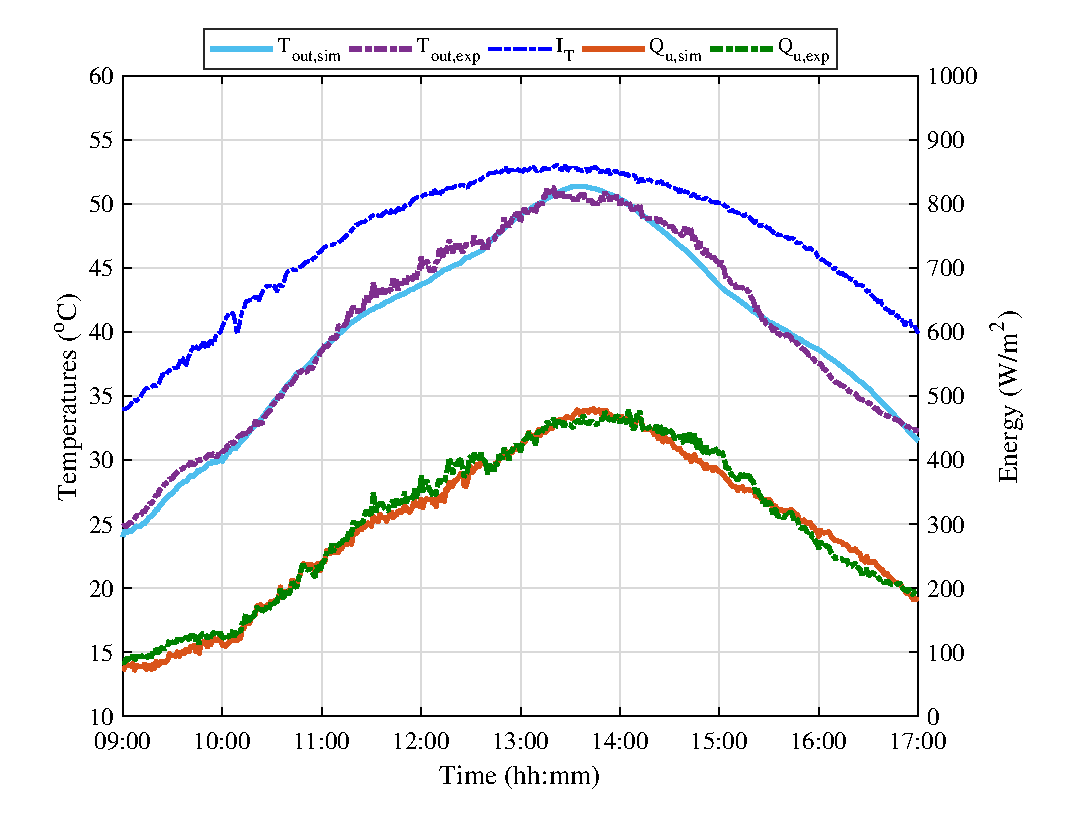
\includegraphics[width=0.99\columnwidth,height=65mm]{figs/004-3.eps}
		%\\[-9mm]
		\subcaption{Experimental and simulated results over time.}
	\end{minipage}
	\begin{minipage}{0.39\columnwidth}
		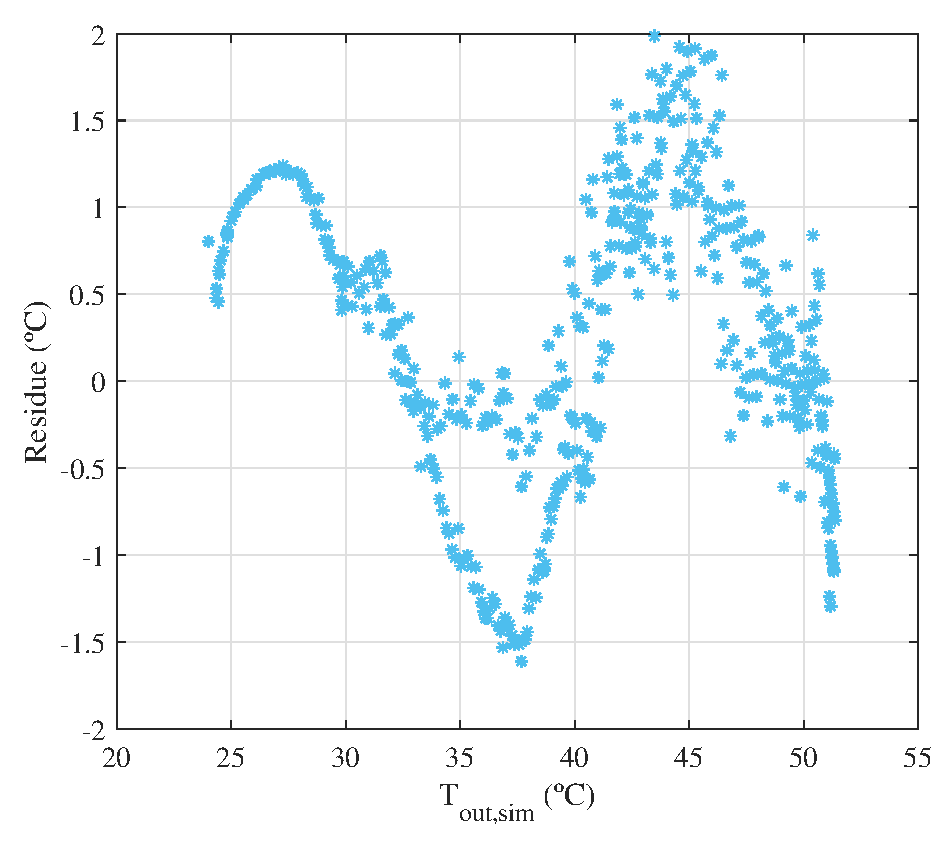
\includegraphics[scale=0.5,width=1.0\columnwidth]{figs/004-residue-5.eps}
		\subcaption{Residue vs. simulated $\rm{T_{out}}$.}
		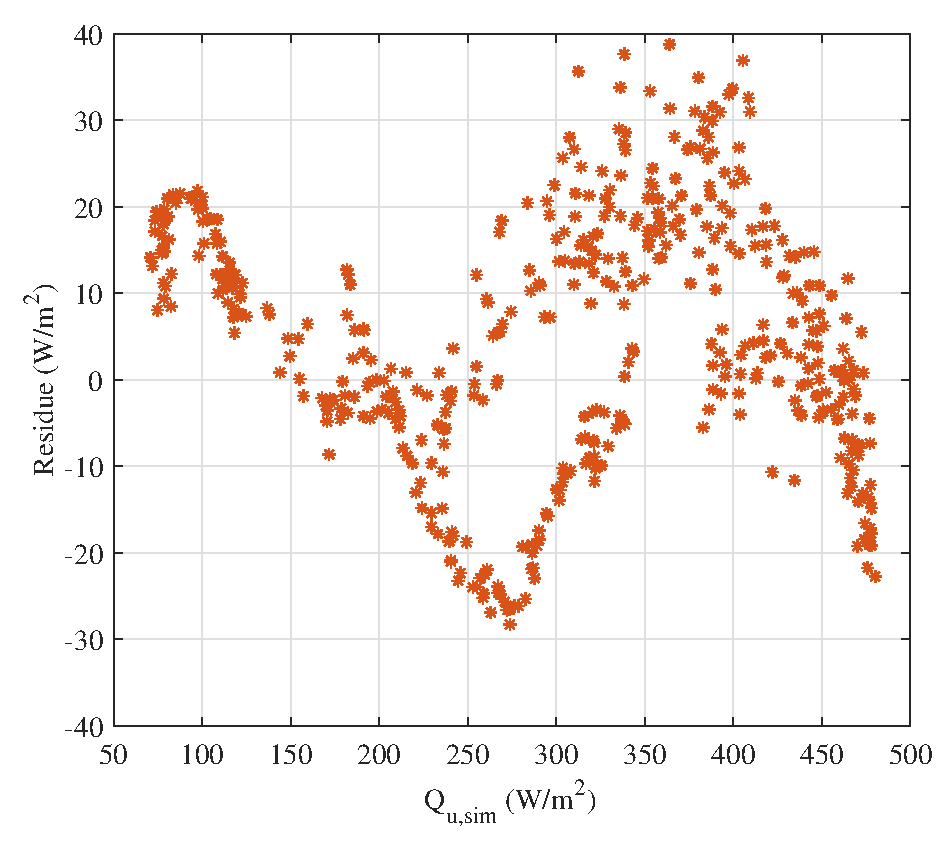
\includegraphics[scale=0.5,width=1.0\columnwidth]{figs/004-residue-6.eps}
		\subcaption{Residue vs. simulated $\rm{Q_{u}}$.}
	\end{minipage}
	
	\caption{(a) Experimental and simulated results, (b) residues of $\rm{T_{out}}$, and (c) residues of $\rm{Q_{u}}$ from 09$^{\rm{th}}$ June at 0.04 kg/(s m$^2$).}
	\label{004-3}
\end{figure}

%\Figure[scale=0.63,placement=!ht,label={004-3},caption={Experimental and simulated results from 09$^{\rm{th}}$ June at 0.04 kg/m$^2$.s. MAE is 2.3\% in terms of $\rm{T_{out}}$ and 7.1\% in terms of $\rm{Q_u}$.}]{figs/004-3.eps}

\newpage
\subsubsection{Validation of results at low-med airflow rate}

Figure \ref{0055-3}(a) shows solar radiation, experimental and simulated data of the test on 22$^{\rm{nd}}$ June ($\rm{G_{air}}$ = 0.055 kg/(s m$^2$)). On this clear sky day with intermittent clouds, the calculated MAE regarding $\rm{T_{out}}$ and $\rm{Q_{u}}$ are 2.2\% and 6.0\%, respectively. Although it was a day with sudden variation in solar radiation at different moments, the model predicted the outputs in which most of the residues are between -0.5 and 1 $^{\rm{o}}$C, and -10 and 30 W/m$^2$, except in two periods: after 16:00, when the decay of $\rm{I_{\!_T}}$ lasted 10 minutes before rising to the natural trend; and shortly before 14:00, when $\rm{I_{\!_T}}$ became highly unstable. These events might explain why the model underestimated the outputs by more than 1.5 $^{\rm{o}}$C and 30 W/m$^2$. From Figures \ref{0055-3}(b) and \ref{0055-3}(c), 85\% of the residues have a magnitude of $\pm$1 $^{\rm{o}}$C;  90\% are between $\pm$30 W/m$^2$ and 88\% of the predictions are underestimated.

%The regions of maximum error is observed in the beginning and in the end of the operation (6\% in $\rm{T_{out}}$ and 20\% in $\rm{Q_u}$). 

\begin{figure}[ht!]
\begin{minipage}{0.60\columnwidth}
		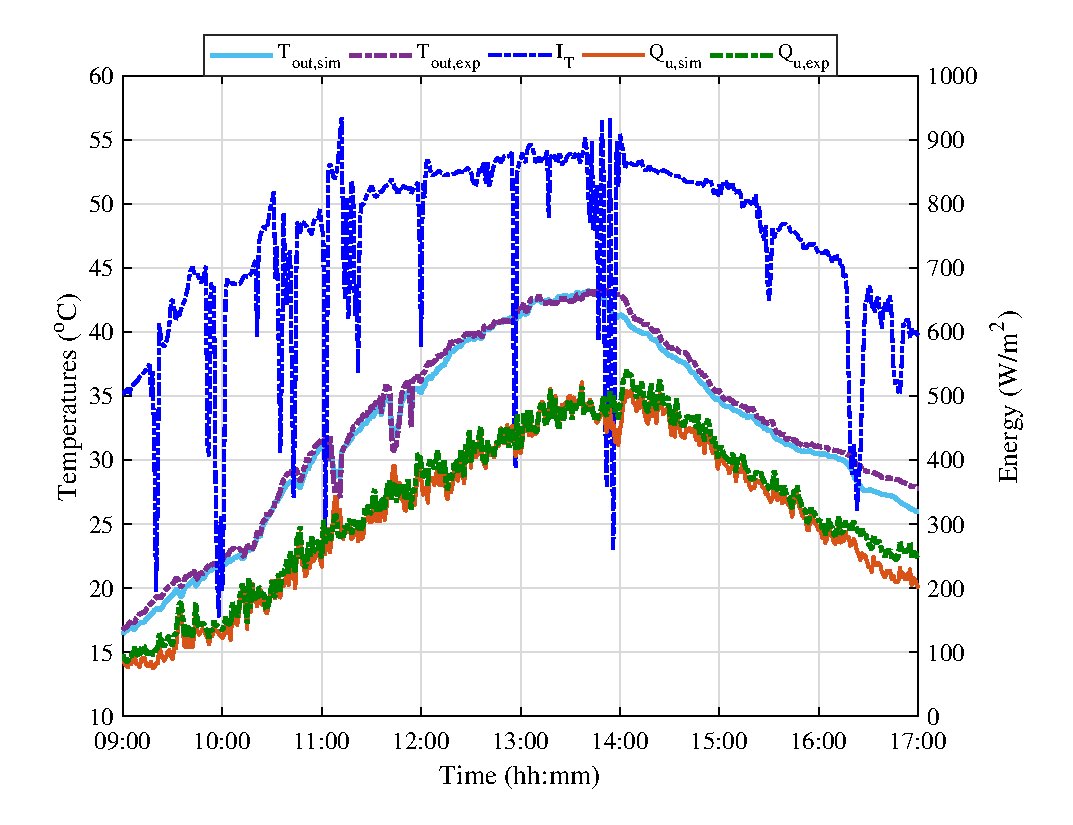
\includegraphics[width=0.99\columnwidth,height=65mm]{figs/0055-3.eps}
		%\\[-9mm]
		\subcaption{Experimental and simulated results over time.}
	\end{minipage}
	\begin{minipage}{0.39\columnwidth}
		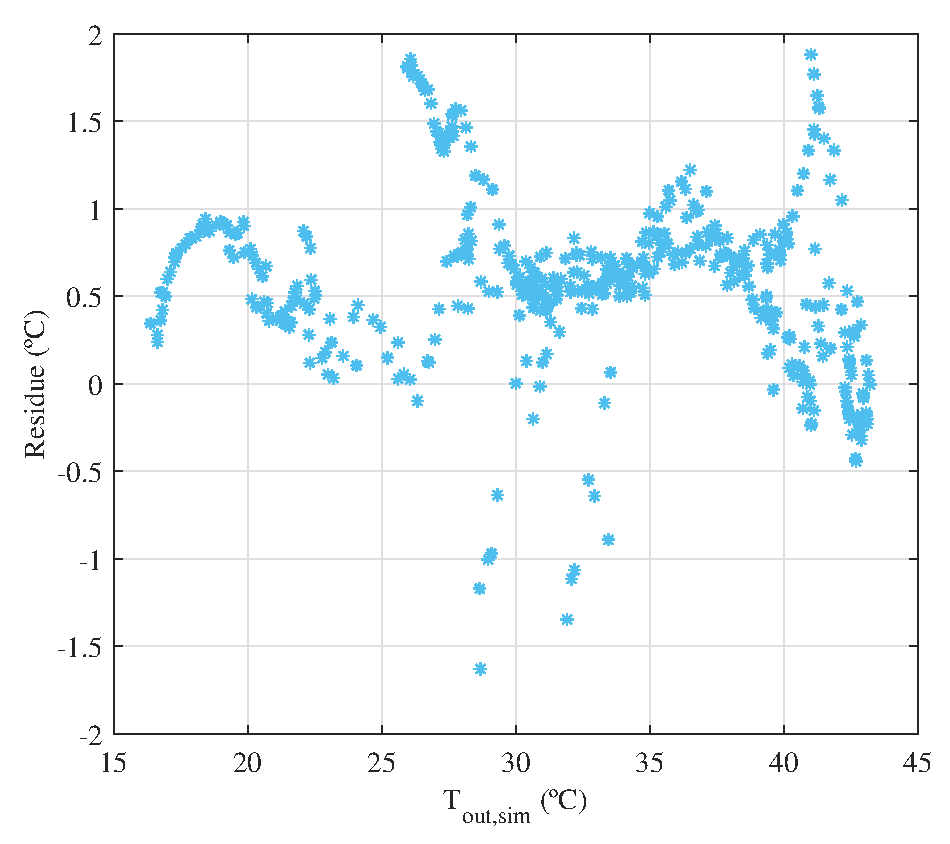
\includegraphics[scale=0.5,width=1.0\columnwidth]{figs/0055-residue-5.eps}
		\subcaption{Residue vs. simulated $\rm{T_{out}}$.}
		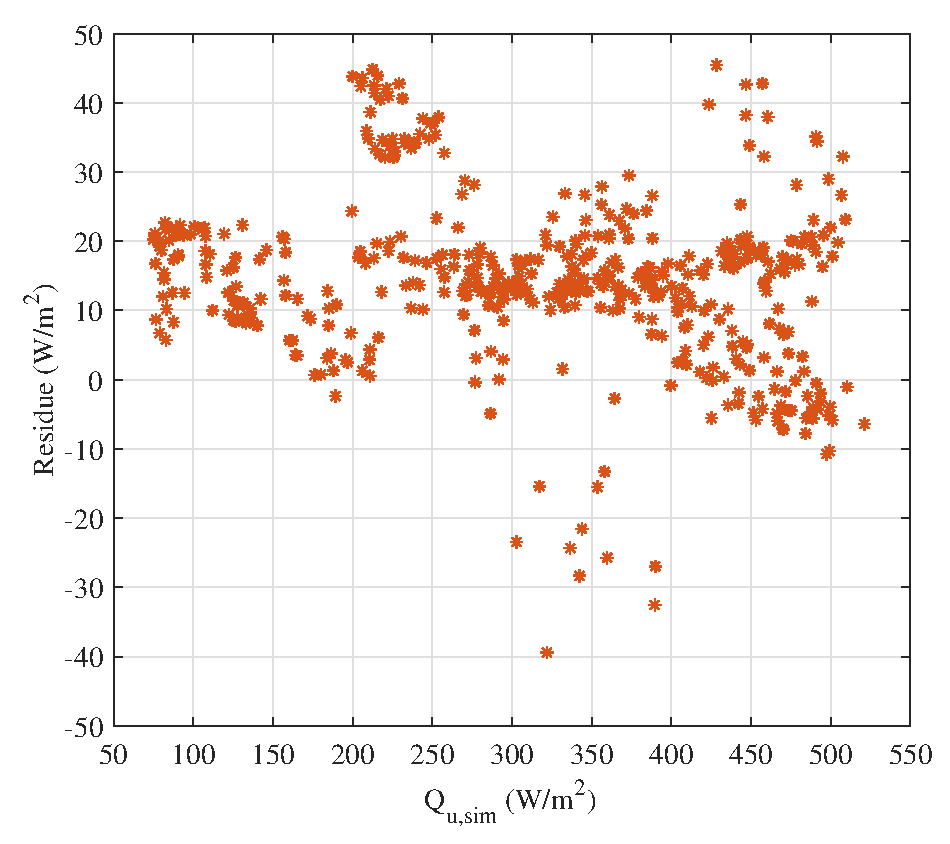
\includegraphics[scale=0.5,width=1.0\columnwidth]{figs/0055-residue-6.eps}
		\subcaption{Residue vs. simulated $\rm{Q_{u}}$.}
	\end{minipage}
	
	\caption{(a) Experimental and simulated results, (b) residues of $\rm{T_{out}}$, and (c) residues of $\rm{Q_{u}}$ from 22$^{\rm{nd}}$ June at 0.055 kg/(s m$^2$).}
	\label{0055-3}
\end{figure}

%\Figure[scale=0.60,placement=!ht,label={0055-3},caption={Experimental and simulated results from 22$^{\rm{nd}}$ June at 0.055 kg/m$^2$.s. MAE is 4.3\% in terms of $\rm{T_{out}}$ and 11.8\% in terms of $\rm{Q_u}$.}]{figs/0055-3.eps}

\subsubsection{Validation of results at medium airflow rate}

Figure \ref{007-3}(a) shows the graphs of solar radiation data, experimental and simulated results of the test on 29$^{\rm{th}}$ May ($\rm{G_{air}}$ = 0.07 kg/m$^2$.s), whereas Figures \ref{007-3}(b) and \ref{007-3}(c) present the residue plot in relation to the simulated values. On this clear sky day with intermittent clouds mainly before 12:00, the calculated MAE for $\rm{T_{out}}$ and $\rm{Q_{u}}$ are 1.6\% and 4.9\%, respectively. The outputs also did not fall substantially due to the sudden variation in solar radiation. In this case, the model underestimated 88\% of the predictions, where 95\% of the residues are between $\pm$1 $^{\rm{o}}$C and 93\% are between $\pm$30 W/m$^2$. It is also noted that the maximum residue is less than 1.2 $^{\rm{o}}$C and less than 40 W/m$^2$. 

\begin{figure}[ht!]
\begin{minipage}{0.60\columnwidth}
		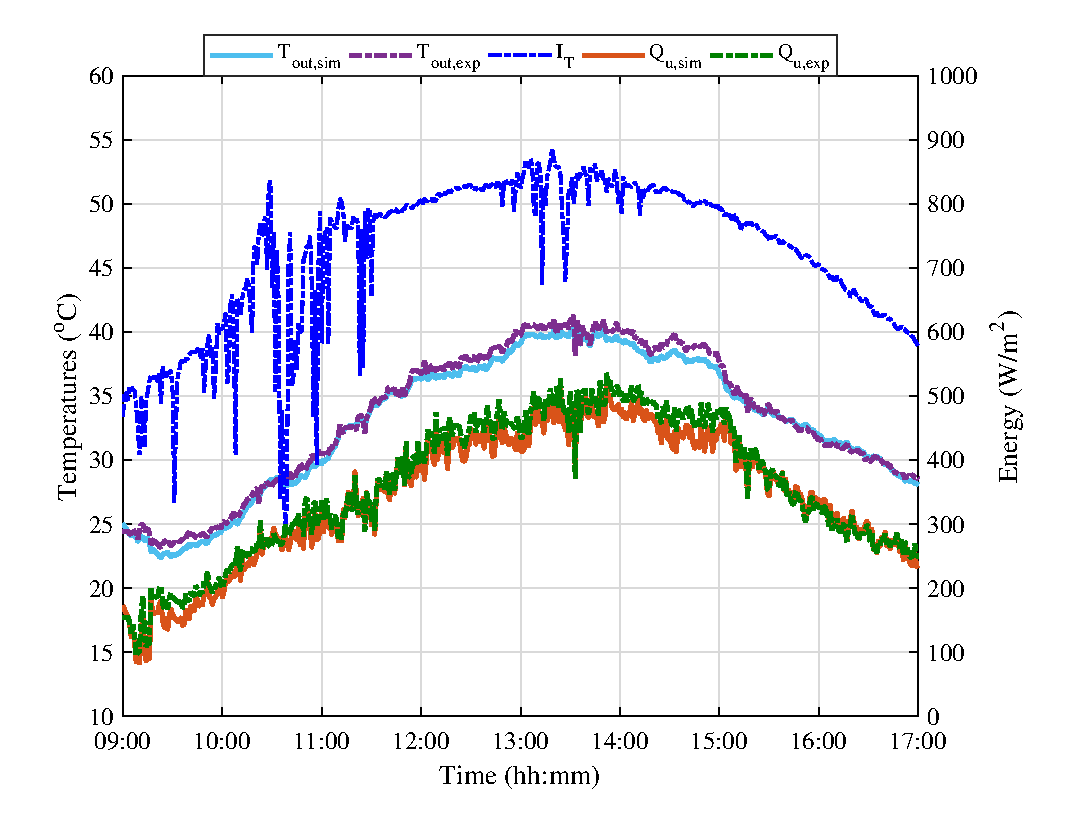
\includegraphics[width=0.99\columnwidth,height=65mm]{figs/007-3.eps}
		%\\[-9mm]
		\subcaption{Experimental and simulated results over time.}
	\end{minipage}
	\begin{minipage}{0.39\columnwidth}
		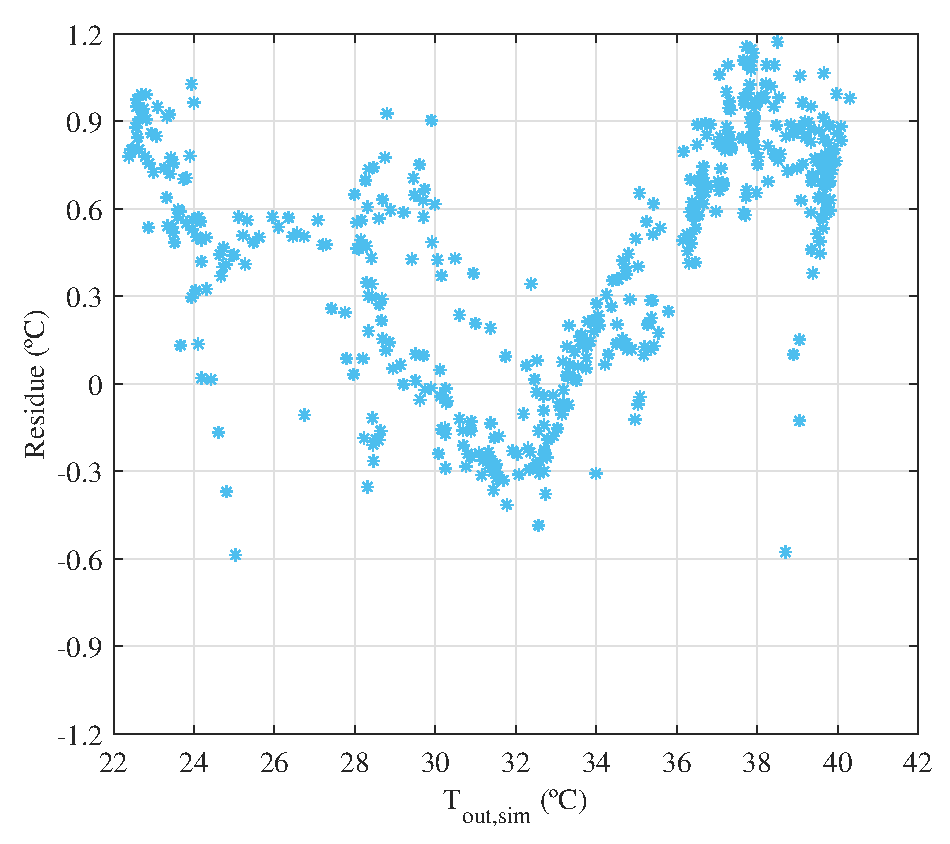
\includegraphics[scale=0.5,width=1.0\columnwidth]{figs/007-residue-5.eps}
		\subcaption{Residue vs. simulated $\rm{T_{out}}$.}
		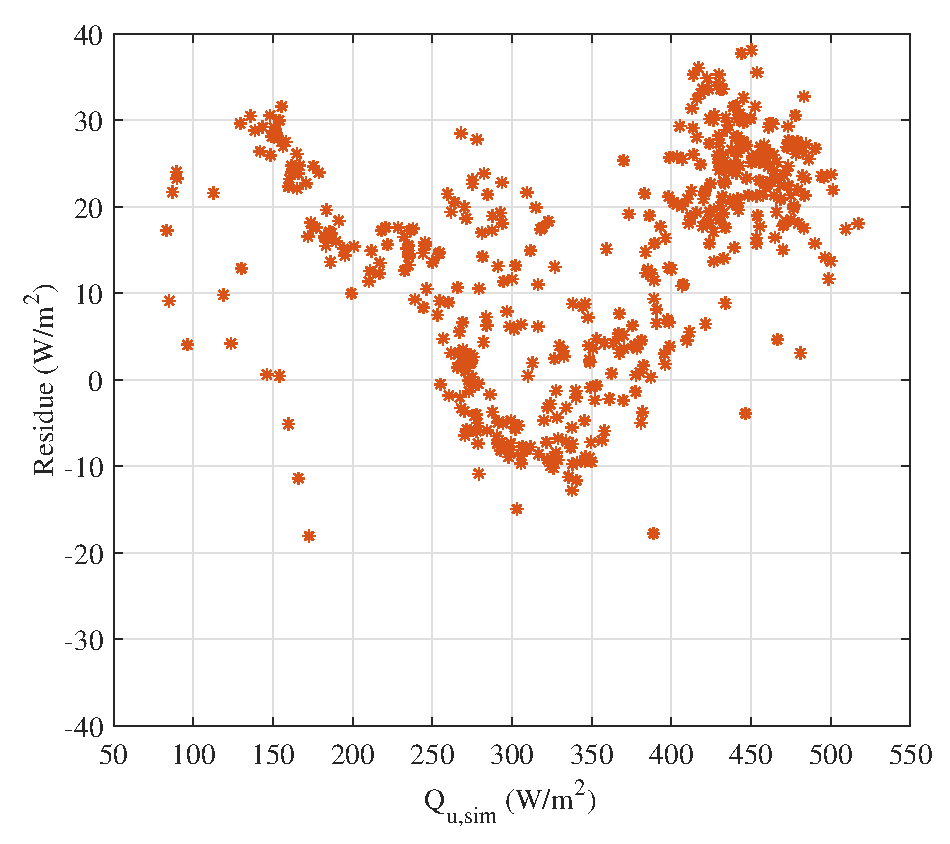
\includegraphics[scale=0.5,width=1.0\columnwidth]{figs/007-residue-6.eps}
		\subcaption{Residue vs. simulated $\rm{Q_{u}}$.}
	\end{minipage}
	
	\caption{(a) Experimental and simulated results, (b) residues of $\rm{T_{out}}$, and (c) residues of $\rm{Q_{u}}$ from 29$^{\rm{th}}$ May at 0.07 kg/(s m$^2$).}
	\label{007-3}
\end{figure}

%\Figure[scale=0.63,placement=!ht,label={007-3},caption={Experimental and simulated results from 29$^{\rm{th}}$ May at 0.07 kg/m$^2$.s. MAE is 6.3\% in terms of $\rm{T_{out}}$ and 19\% in terms of $\rm{Q_u}$.}]{figs/007-3.eps}

\newpage
\subsubsection{Validation of results at medium-high airflow rate}

Figure \ref{009-3}(a) shows solar radiation, experimental and simulated data of the test on 29$^{\rm{th}}$ May ($\rm{G_{air}}$ = 0.09 kg/m$^2$.s). The calculated MAE for $\rm{T_{out}}$ and $\rm{Q_{u}}$ are 2.5\% and 13.7\%, respectively. The model prediction is the least accurate in this case due to high variations in $\rm{I_{\!_T}}$ throughout the day. From 14:00 to 15:00, the model overestimated the experimental data by more than 2 $^{\rm{o}}$C, more than 56 W/m$^2$ and up to 130 W/m$^2$. This large difference can be due to any unknown experimental fluctuation during the test. From Figures \ref{009-3}(b) and \ref{009-3}(c), the simulated outputs were also underestimated compared to the experimental results in 79\% of the cases. It was found that 70\% of the residues have a magnitude of \mbox{$\pm$1 $^{\rm{o}}$C} and 75\% are between $\pm$40 W/m$^2$.

\begin{figure}[ht!]
\begin{minipage}{0.60\columnwidth}
		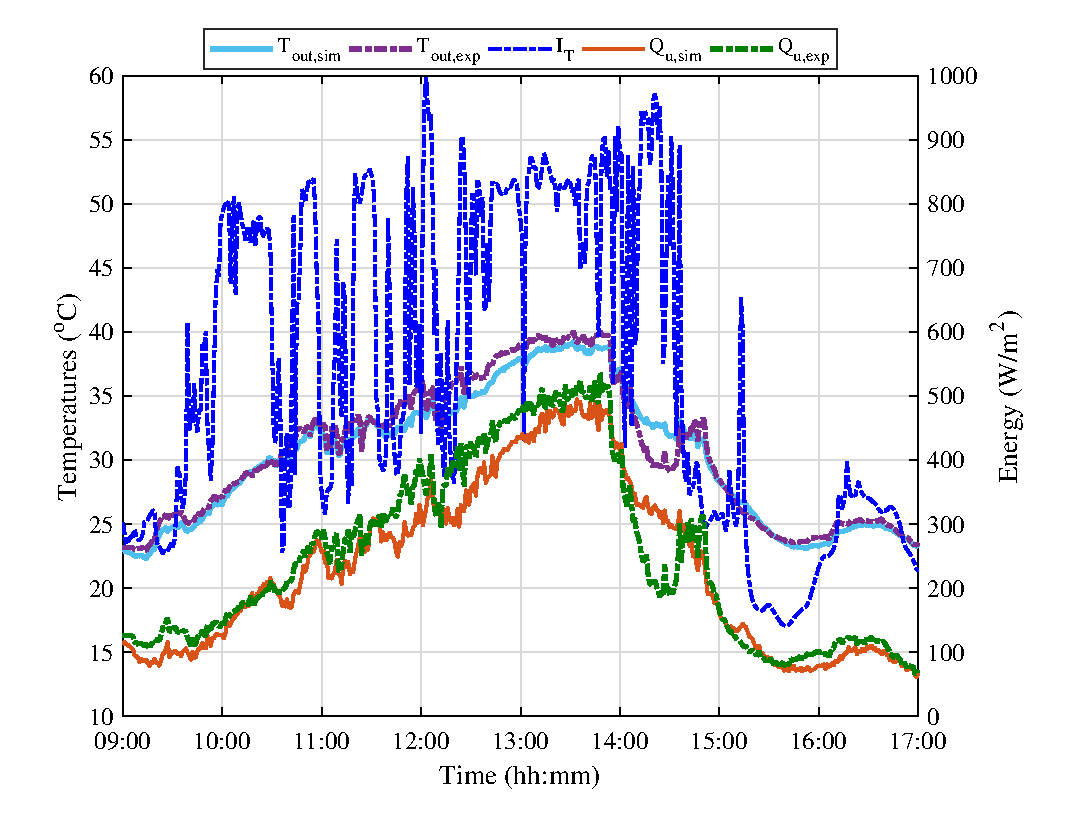
\includegraphics[width=0.99\columnwidth,height=65mm]{figs/009-3.eps}
		%\\[-9mm]
		\subcaption{Experimental and simulated results over time.}
	\end{minipage}
	\begin{minipage}{0.39\columnwidth}
		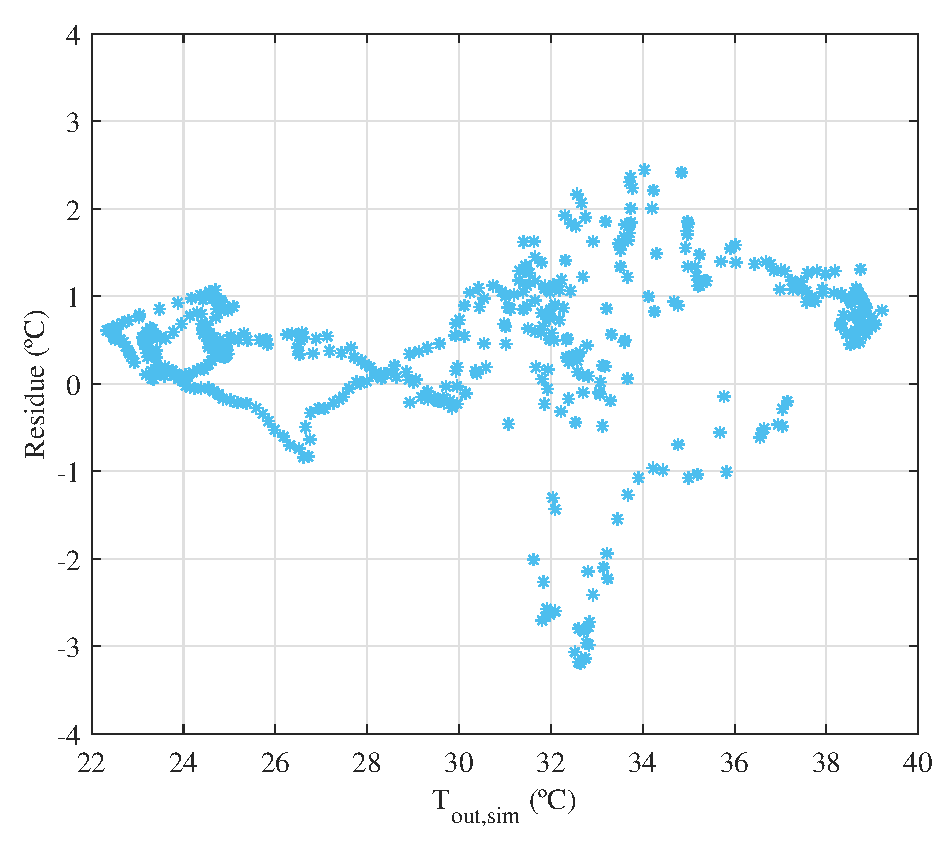
\includegraphics[scale=0.5,width=1.0\columnwidth]{figs/009-residue-5.eps}
		\subcaption{Residue vs. simulated $\rm{T_{out}}$.}
		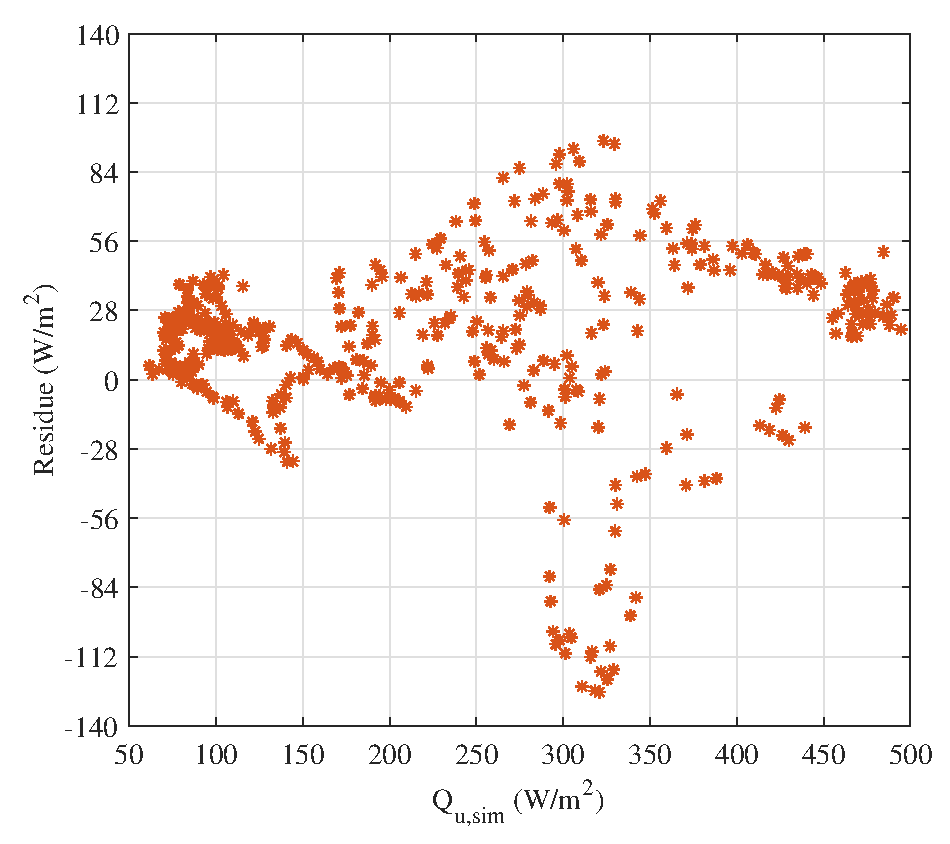
\includegraphics[scale=0.5,width=1.0\columnwidth]{figs/009-residue-6.eps}
		\subcaption{Residue vs. simulated $\rm{Q_{u}}$.}
	\end{minipage}
	
	\caption{Experimental and simulated results from 31$^{\rm{st}}$ May at 0.09 kg/(s m$^2$).}
	\label{009-3}
\end{figure}

%\Figure[scale=0.63,placement=!ht,label={009-3},caption={Experimental and simulated results from 31$^{\rm{st}}$ May at 0.09 kg/m$^2$.s. MAE is 4.9\% in terms of $\rm{T_{out}}$ and 27.5\% in terms of $\rm{Q_u}$.}]{figs/009-3.eps}

\subsubsection{Validation of results at high airflow rate}

Figure \ref{0115-3}(a) shows the graphs of solar radiation data, experimental and simulated results of the test on 28$^{\rm{th}}$ June ($\rm{G_{air}}$ = 0.115 kg/(s m$^2$), whereas Figures \ref{0115-3}(b) and \ref{0115-3}(c) present the residue plot in relation to the simulated values. On this clear sky day, the calculated MAE for $\rm{T_{out}}$ and $\rm{Q_{u}}$ are 1.1\% and 7.0\%, respectively. In this case, the model underestimated 78\% of the predictions, where 83\% of the residues are between $\pm$0.6 $^{\rm{o}}$C and 83\% was between $\pm$30 W/m$^2$. After 14:00, the model mostly underestimated $\rm{Q_{u}}$ by 20 to 40 W/m$^2$. It is also noticed that the maximum residue is less than 1.0 $^{\rm{o}}$C and less than 40 W/m$^2$.

\begin{figure}[ht!]
\begin{minipage}{0.60\columnwidth}
		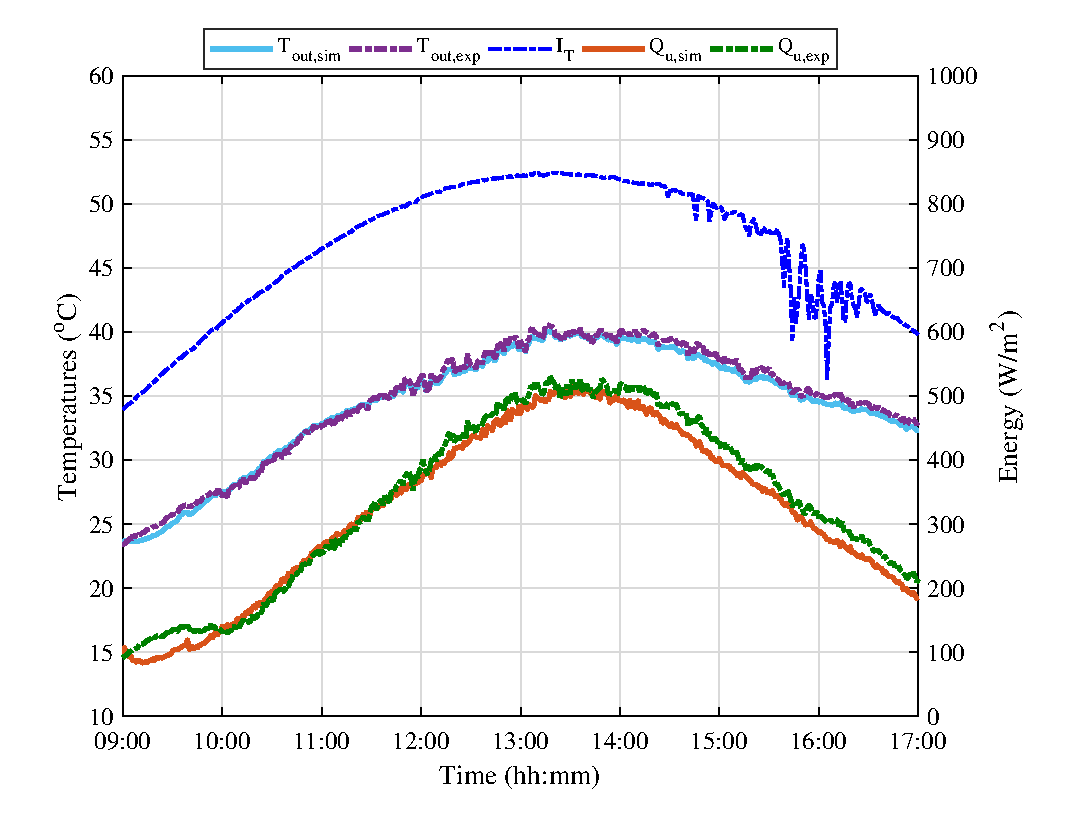
\includegraphics[width=0.99\columnwidth,height=65mm]{figs/0115-3.eps}
		%\\[-9mm]
		\subcaption{Experimental and simulated results over time.}
	\end{minipage}
	\begin{minipage}{0.39\columnwidth}
		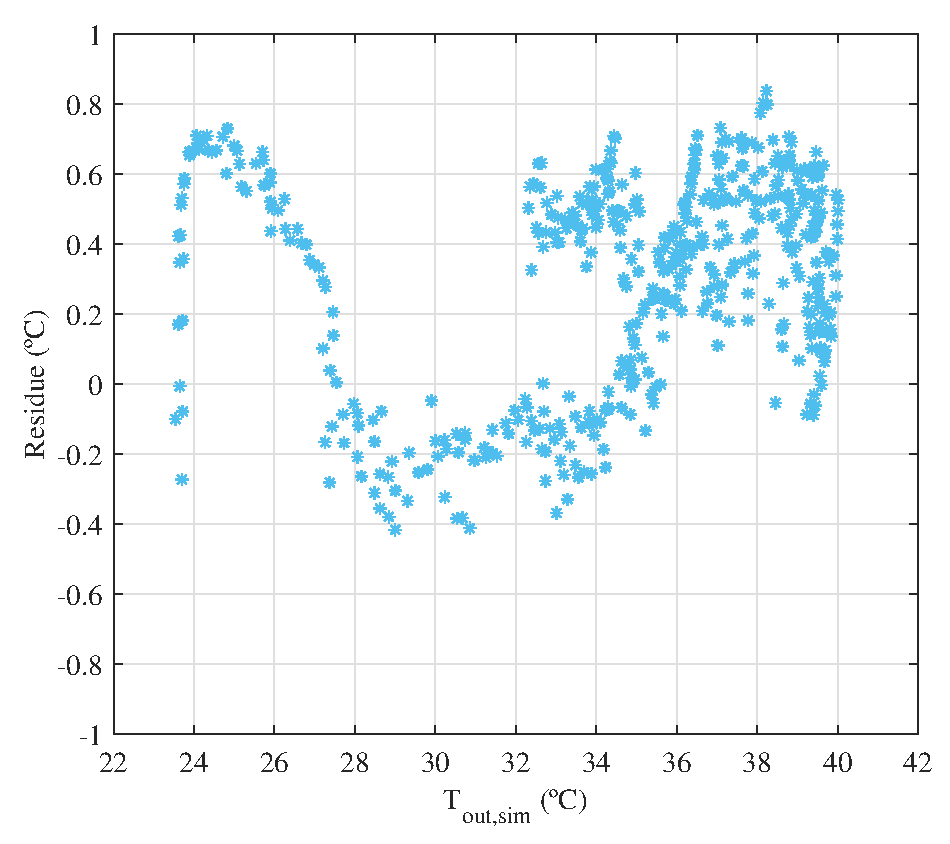
\includegraphics[scale=0.5,width=1.0\columnwidth]{figs/0115-residue-5.eps}
		\subcaption{Residue vs. simulated $\rm{T_{out}}$.}
		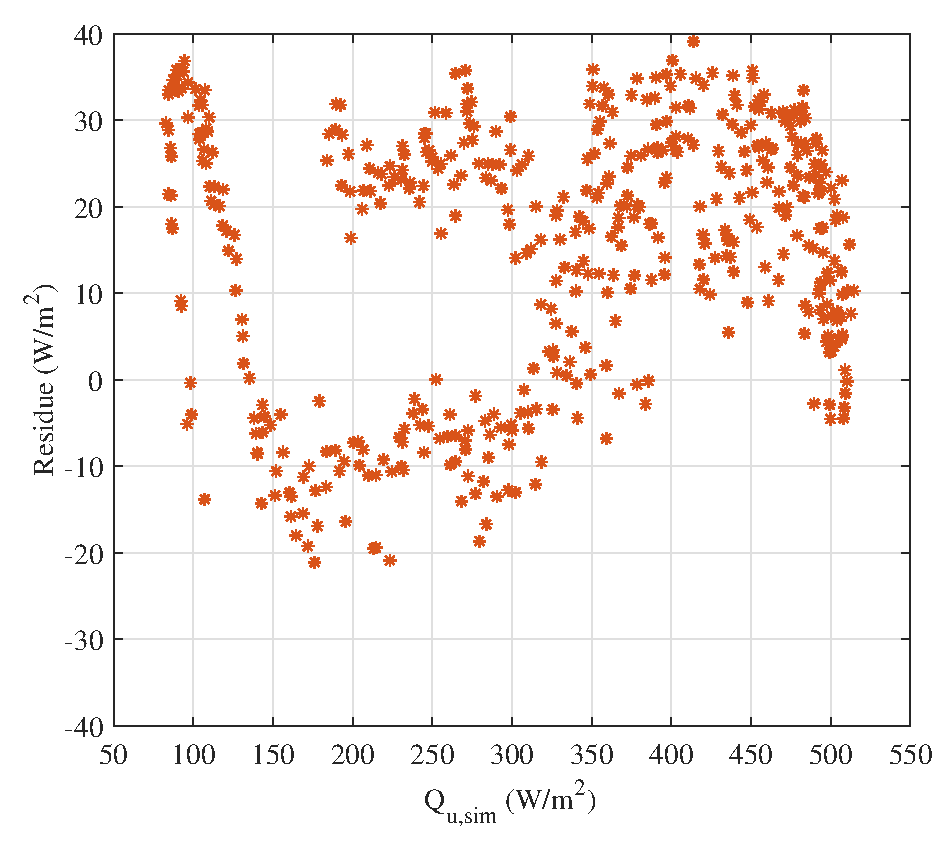
\includegraphics[scale=0.5,width=1.0\columnwidth]{figs/0115-residue-6.eps}
		\subcaption{Residue vs. simulated $\rm{Q_{u}}$.}
	\end{minipage}
	
	\caption{(a) Experimental and simulated results, (b) residues of $\rm{T_{out}}$, and (c) residues of $\rm{Q_{u}}$ from 28$^{\rm{th}}$ June at 0.115 kg/(s m$^2$).}
	\label{0115-3}
\end{figure}

%\Figure[scale=0.63,placement=!ht,label={0115-3},caption={Experimental and simulated results from 28$^{\rm{th}}$ June at 0.115 kg/m$^2$.s. MAE is 2.2\% in terms of $\rm{T_{out}}$ and 14\% in terms of $\rm{Q_u}$.}]{figs/0115-3.eps}

\newpage
Hence, from the calculated MAE and residue plots, there was no effect of the airflow rate and time of operation on the model prediction. To check if solar radiation influences the model prediction, all residues were plotted against $\rm{I_{\!_T}}$, as shown in Figure \ref{res_it}. It can be seen that the residues are concentrated in the region of $\rm{I_{\!_T}}$ above 600 W/m$^2$, and most of them are between $\pm$2.0 $^{\rm{o}}$C and $\pm$50 W/m$^2$. The highest residues were observed for days with high intermittent clouds.

\begin{figure}[ht!]
	\begin{minipage}{0.49\columnwidth}
		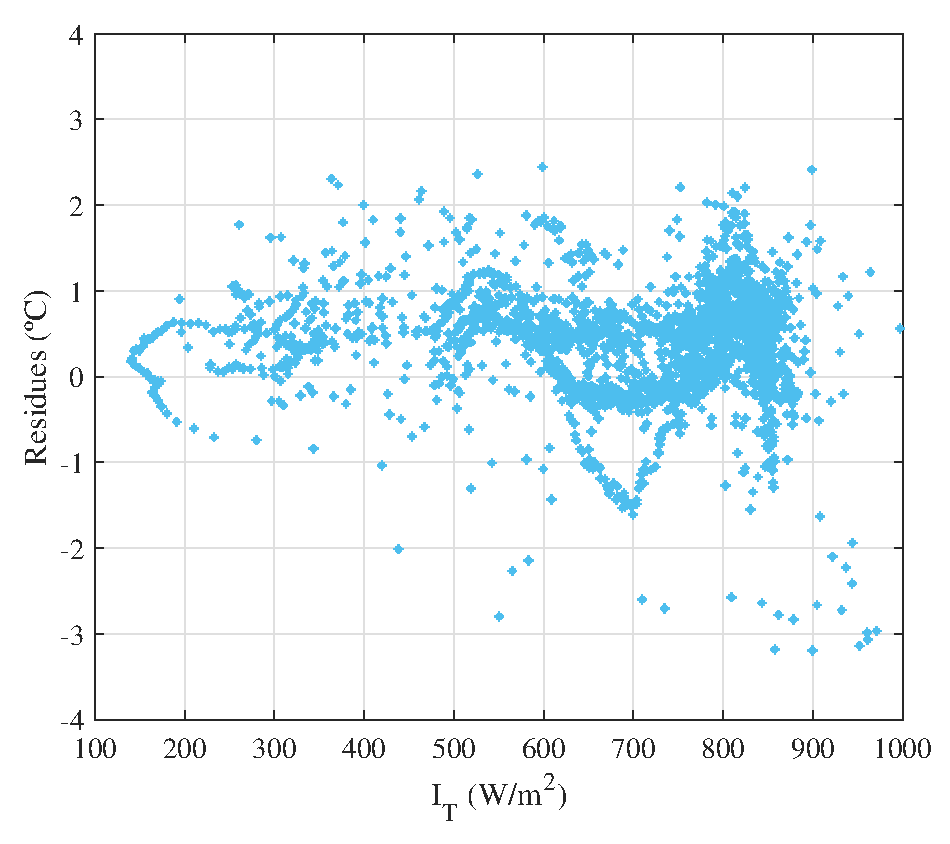
\includegraphics[width=0.95\columnwidth,height=5.5cm]{figs/residueT_it.eps}
		\subcaption{Residue vs. solar radiation for $\rm{T_{out}}$.}
	\end{minipage}
	\begin{minipage}{0.49\columnwidth}
		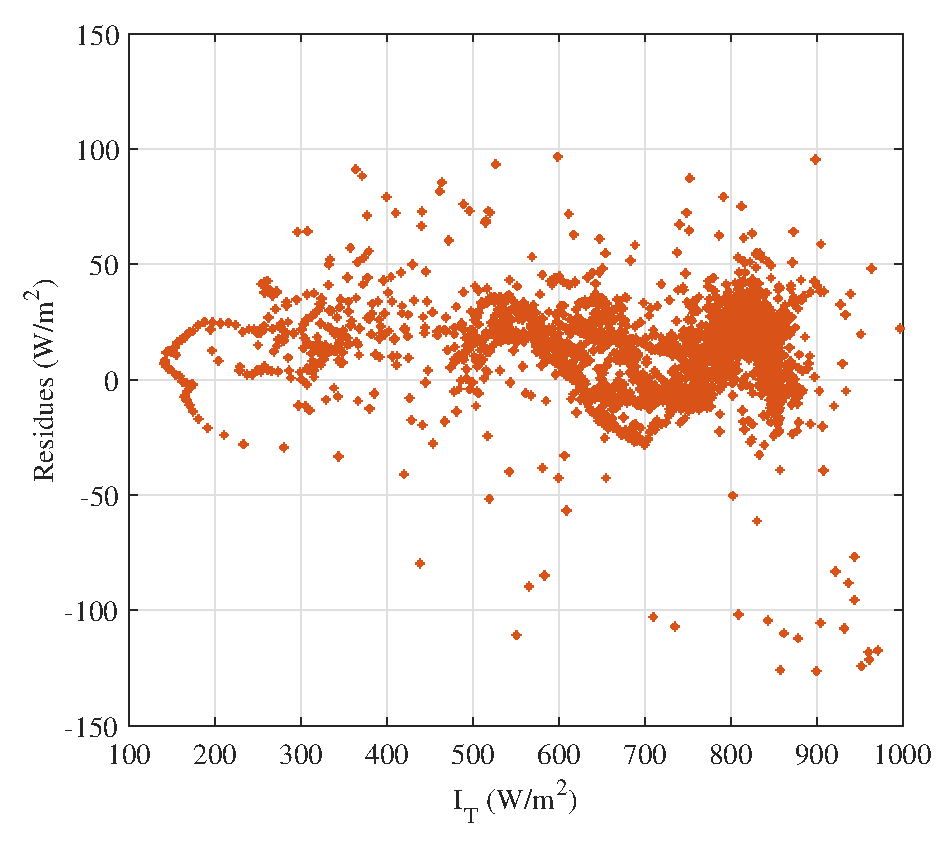
\includegraphics[width=1.0\columnwidth,height=5.5cm]{figs/residueQ_it.eps}
		\subcaption{Residue vs. solar radiation for $\rm{Q_u}$.}
	\end{minipage}
	\caption{Residues vs. solar radiation for (a) $\rm{T_{out}}$, and (b) $\rm{Q_u}$.}
	\label{res_it}
\end{figure}

Another way to analyse these residue data is by plotting the cumulative frequency distribution of each simulated output, as shown in Figure \ref{cdf}. From the cumulative distributions, 95\% of the data predicted have residues between $\pm$2 $^{\rm{o}}$C and $\pm$50 W/m$^{2}$C. It was also found that 65\% of the predictions are underestimated, which highlights the underestimation of the simulation results most of the time.

\begin{figure}[ht!]
	\begin{minipage}{0.49\columnwidth}
		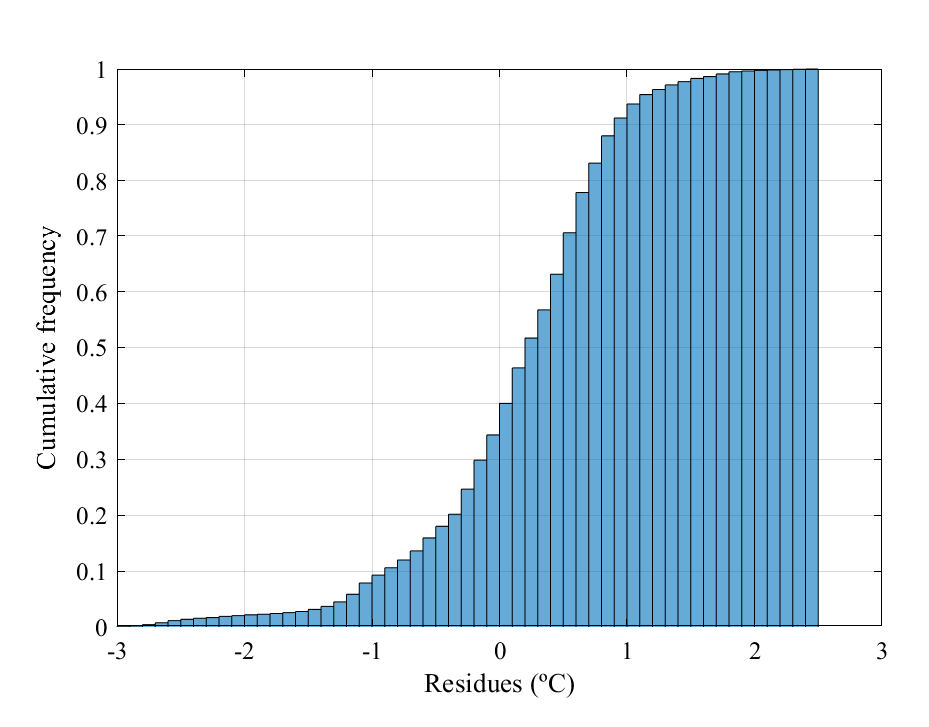
\includegraphics[width=0.95\columnwidth,height=5.5cm]{figs/cdf_T.eps}
		\subcaption{Cumulative frequency of residues from $\rm{T_{out}}$.}
	\end{minipage}
	\begin{minipage}{0.49\columnwidth}
		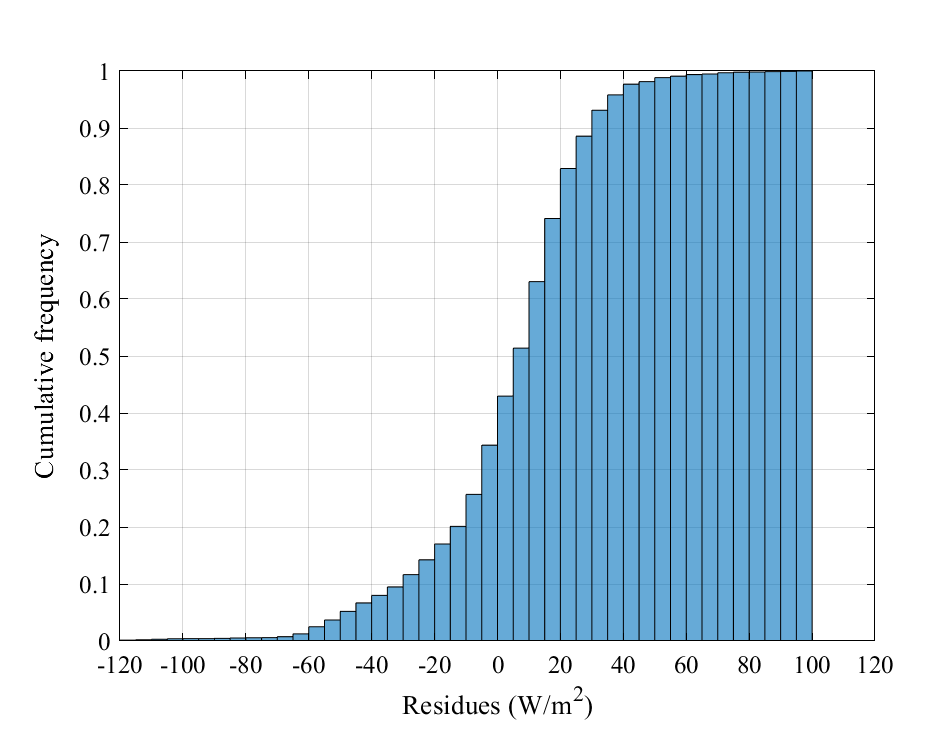
\includegraphics[width=1.0\columnwidth,height=5.5cm]{figs/cdf_Q.eps}
		\subcaption{Cumulative frequency of residues from $\rm{Q_u}$.}
	\end{minipage}
	\caption{Residual cumulative frequency distribution of (a) $\rm{T_{out}}$, and (b) $\rm{Q_u}$.}
	\label{cdf}
\end{figure}


\section{Thermal characterisation from simulation results}

After validation, the heat transfer model characterised the system's thermal performance under clear sky days at a transient state. The input ranges of which this system can be modelled, are depicted as follows:

\begin{description}
	\item[Solar radiation:] 500 -- 1000 W/m$^2$, where the lowest limit corresponds to the airflow temperature increase at the beginning of the operation;
	\item[Mass airflow rate:] 0.04 -- 0.12 kg/(s m$^2$), where the limits are coincident to the ones of the tests;
	\item[Ambient temperature:] 20 -- 30 $^{\rm{o}}$C, which includes all the measured data on clear sky days;
	\item[Wind speed:] 0 -- 10 m/s, including all the data taken from the Met Eireann website.
\end{description}

%In the first scenario,

%The parameters $\rm{T_{amb}}$, $\rm{v_w}$ and $\rm{I_{\!_T}}$ were kept constant during the simulations regardless the amount of beam and diffuse components, which allows to assume that $\gamma = $1.





%\begin{table}[!ht]
%	\caption{Input values for simulation}
%	\centering
%	\begin{tabular}{p{5.1cm}p{3.7cm}}
%		\hline \\[-10pt] 
%		\rule[-1ex]{0pt}{2.5ex} Model Input & Value/Range \\ [3pt]
%		\hline \\[-10pt]
%		\rule[-1ex]{0pt}{2.5ex} Total solar radiation ($\rm{I_{\!_T}}$) & 500 -- 1000 W/m$^2$ \\ [5pt]
%		\rule[-1ex]{0pt}{2.5ex} Ambient temperature ($\rm{T_{amb}}$) & 20 -- 30 $\rm{^o}$C \\ [5pt] 
%		\rule[-1ex]{0pt}{2.5ex} Wind speed ($\rm{v_w}$) & 0 -- 10 m/s \\ [5pt]
%		\rule[-1ex]{0pt}{2.5ex} Inlet air temperature ($\rm{T_{in}}$) & 20 -- 30 $\rm{^o}$C  \\ [5pt]
%		\rule[-1ex]{0pt}{2.5ex} Airflow rate ($\rm{G_{air}}$) & 0.04 -- 0.12 kg/(m$^2$.s)  \\ [5pt]
%		%\rule[-1ex]{0pt}{2.5ex} Optical efficiency ($\eta_{\rm{o}}$) & Eq. (\ref{optHts}) \\ 
%		
%		\hline 
%	\end{tabular} 
%	\label{inputs}
%\end{table}

\subsection{Thermal performance of a single collector}

To characterise this air heating system with a single collector, a particular clear sky day (30$^{\rm{th}}$ June) was taken to represent the results. The simulation was performed at the five different airflow rates and the correspondent graphs of $\rm{T_{out}}$ were plotted in Figure \ref{Touts_sim}. All the temperature profiles reached their maximum levels in the hour of highest solar radiation ($\rm{I_{\!_T}}$ = 860 W/m$^2$). 

\Figure[scale=0.69,placement=!ht,label={Touts_sim},caption={Simulated $\rm{T_{out}}$ at the five different airflow rates used in the tests under conditions of 30$^{\rm{th}}$ June.}]{figs/series_1st.eps}

With the simulation data obtained, Figure \ref{Tout-IT-Gair} presents the surface and contour plot to fit the air temperature rise ($\Delta \rm{T}$) as a function of the solar radiation and airflow rate. Overall, an increase in air temperature is observed from $\rm{I_{\!_T}}$ above 500 W/m$^2$ and increases in a nearly linear way as more energy comes into the system. The opposite effect is noticed as the airflow is increased because $\Delta \rm{T}$ is inversely proportional to $\rm{G_{air}}$. Temperature rises above 27 $^{\rm{o}}$C can be obtained at airflow rate of 0.04 kg/(s m$^2$) when $\rm{I_{\!_T}}$ is above \mbox{860 W/m$^2$}.

\begin{figure}[ht!]
	\begin{minipage}{0.49\columnwidth}
		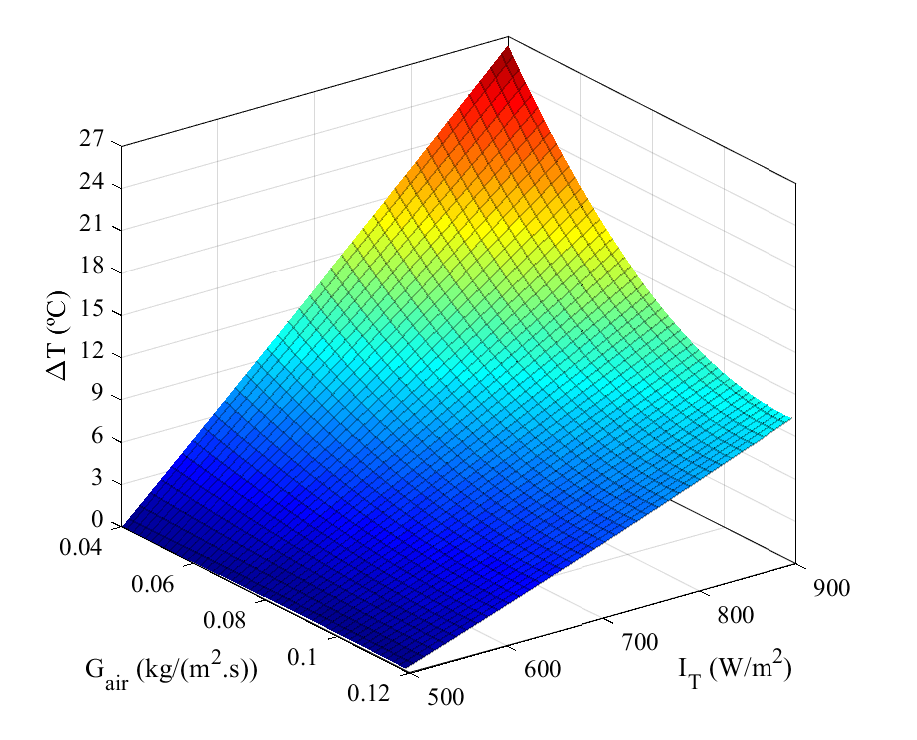
\includegraphics[scale=0.49]{figs/Tout_x_GT_Gair.eps}
		\subcaption{Surface plot.}
	\end{minipage}
	\begin{minipage}{0.49\columnwidth}
		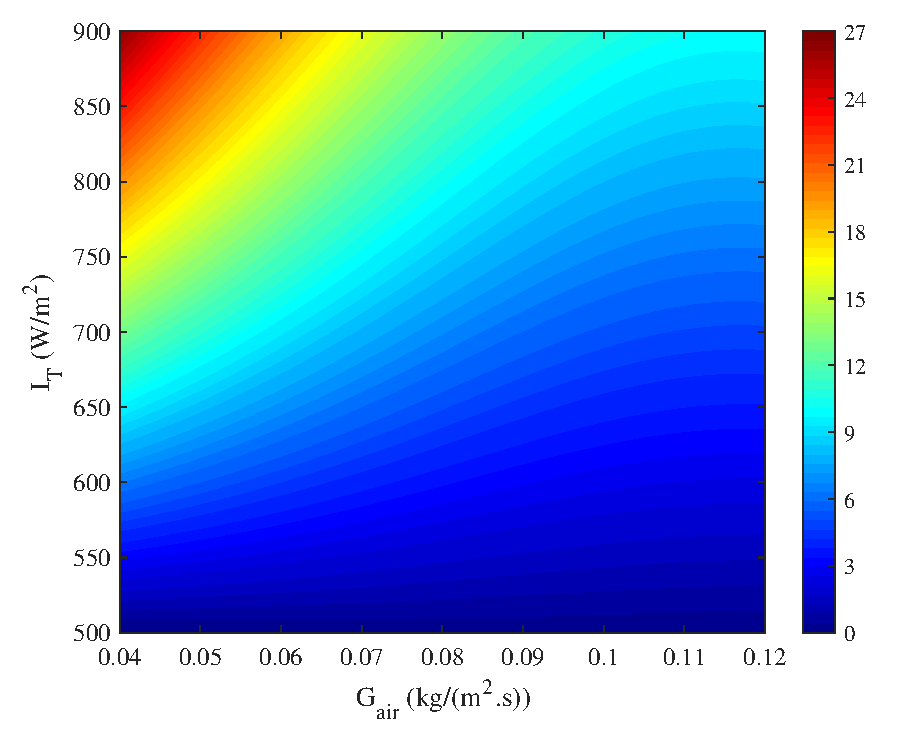
\includegraphics[scale=0.49]{figs/contour_dT.eps}
		\subcaption{Contour plot.}
	\end{minipage}
	\caption{(a) Surface and (b) contour plot of air temperature rise vs. solar radiation and airflow rate.}
	\label{Tout-IT-Gair}
\end{figure}

%\Figure[scale=0.60,placement=!ht,label={Tout-IT-Gair},caption={Surface plot of air temperature rise vs. solar radiation and airflow rate.}]{figs/Tout_x_GT_Gair.eps}

\newpage
To express these results in terms of useful energy, Figure \ref{QU-Tout-Gair} shows this output's surface and contour plot against air temperature rise and airflow rate. $\rm{Q_u}$ increases as $\rm{G_{air}}$ and $\Delta \rm{T}$ become higher, directly proportional to both inputs. The temperature increases more at lower airflow rates but at the cost of delivering a low useful energy, highlighting the trade-off between energy collected and outlet air temperature.

\begin{figure}[ht!]
	\begin{minipage}{0.49\columnwidth}
		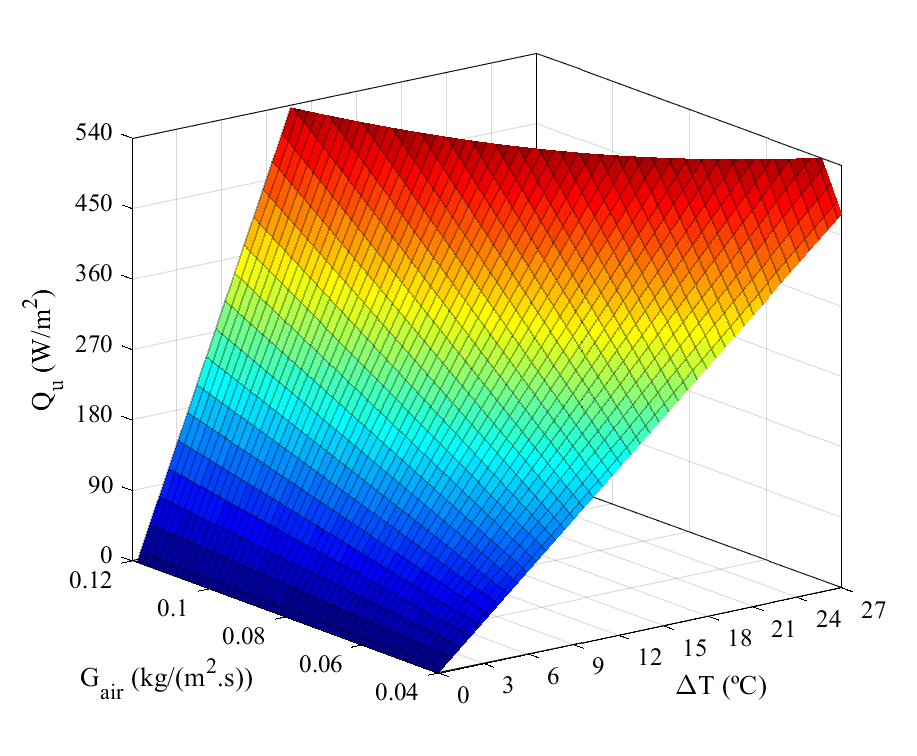
\includegraphics[scale=0.48]{figs/QU_Tout_Gair.eps}
		\subcaption{Surface plot.}
	\end{minipage}
	\begin{minipage}{0.49\columnwidth}
		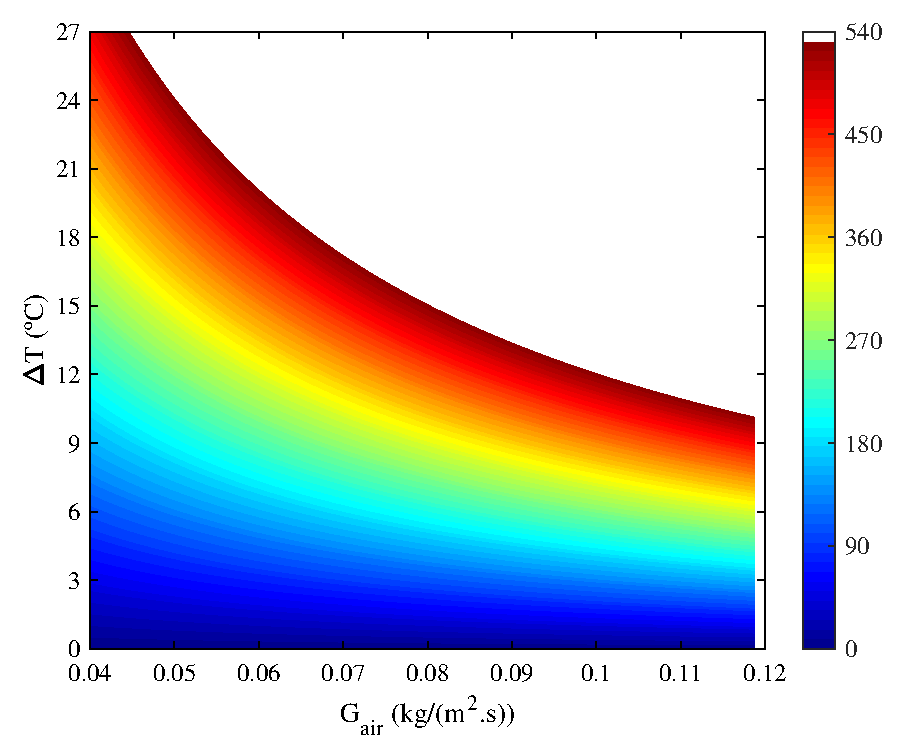
\includegraphics[scale=0.48]{figs/contour_Q.eps}
		\subcaption{Contour plot.}
	\end{minipage}
	\caption{(a) Surface and (b) contour plot of useful energy vs. air temperature rise and airflow rate.}
	\label{QU-Tout-Gair}
\end{figure}

%\Figure[scale=0.60,placement=!ht,label={QU-Tout-Gair},caption={Surface plot of useful energy rate vs. air temperature rise and airflow rates.}]{figs/QU_Tout_Gair.eps}

Figure \ref{ef_curve2} shows simulated data taken under the same conditions depicted in Chapter \ref{Cap:Exp} at nearly steady state. Comparing the parameters of the Hottel-Whillier-Bliss equation, $\rm{F_{\!_R}}\eta_{\rm{o}}$ and $\rm{ F_{\!_R}{U_{\!_L}}}$ calculated by the thermal model are 0.64 and -3.02, respectively, with relative differences of 2\% and 10\% in relation to the parameters of the experimental data. The coefficient of correlation  of the simulated curve is 0.9.

\Figure[scale=0.65,placement=!ht,label={ef_curve2},caption={Experimental and simulated thermal efficiency curves.}]{figs/ef_curve2.eps}

\subsection{Simulation of three connected collectors}

The thermal performance of three interconnected collectors was analysed with regard to their connection in series and parallel configurations. The reason for selecting three collectors in this simulation is their total aperture height of approximately 1 meter when stacked above one another on a wall.

\subsubsection{Connection in series}

Figure \ref{D-series} illustrates the frontal view drawing of the collectors arranged in series. In this configuration, the airflow enters the system through the labelled inlet duct and exits through the indicated outlet duct. The drawing indicates that the airflow leaving the first collector (IACPC 1) immediately enters the second collector (IACPC 2) at its right end, while the airflow leaving IACPC 2 enters the third collector (IACPC 3) at its left end.

\Figure[scale=0.70,placement=!ht,label={D-series},caption={Frontal view of three collectors connected in series.}]{figs/Drawing-Series.png}

The outlet air temperature profiles at four different airflow levels throughout the time of operation for the other two collectors are shown in Figure \ref{Temp-series}, where the results are for (a) the second collector, and (b) for the third one.

\begin{figure}[ht!]
	\begin{minipage}{0.49\columnwidth}
		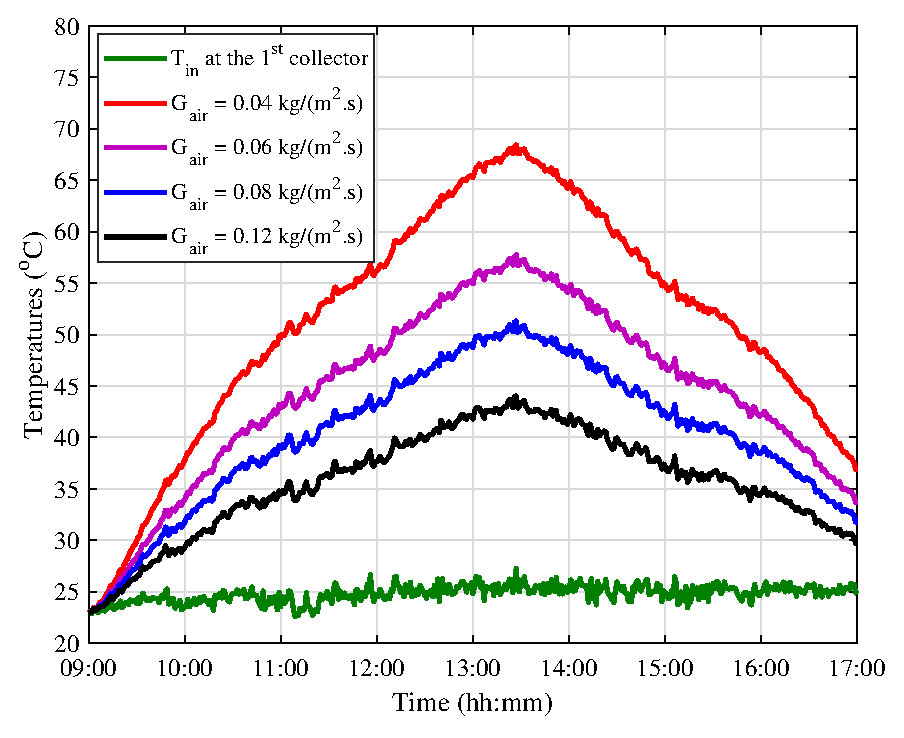
\includegraphics[scale=0.49]{figs/series_2nd.eps}
		\subcaption{Simulation results for the second collector.}
		
	\end{minipage}
	\begin{minipage}{0.49\columnwidth}
		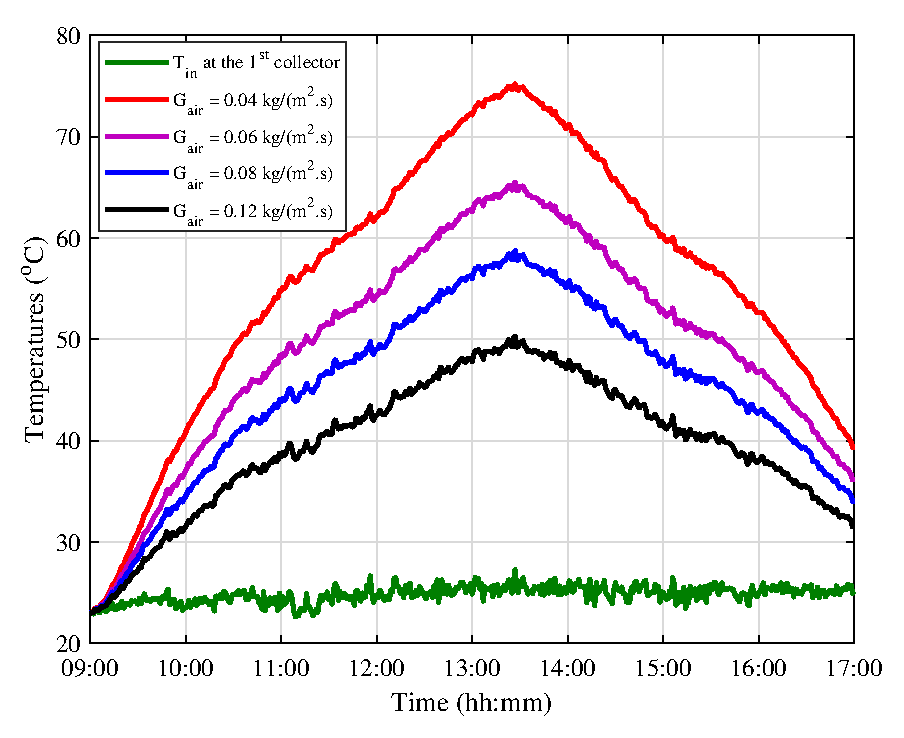
\includegraphics[scale=0.49]{figs/series_3rd.eps}
		\subcaption{Simulation results for the third collector.}
		
	\end{minipage}
	\caption{Simulated $\rm{T_{out}}$ at four different airflow rates for connection in series.}
	\label{Temp-series}
\end{figure}

Figure \ref{series2} shows the useful heat and the mean air temperature at noon hour as a function of the airflow rate leaving each collector. The maximum mean $\rm{T_{out}}$ of the system is 72 $^{\rm{o}}$C for the lowest level of $\rm{G_{air}}$. On the other hand, the highest $\rm{G_{air}}$ can collect the highest $\rm{Q_{u}}$ value of 21.5 MJ/m$^{\rm 2}$ in total and deliver a mean temperature at noon of 48~$^{\rm{o}}$C. It is important to mention that the highest airflow rate can deliver approximately the same outlet air temperature as the system, which consists of a standalone collector at the lowest airflow rate. However, the three-collector system collects 3 times more useful heat.

\Figure[scale=0.65,placement=!ht,label={series2},caption={Total useful heat and mean $\rm{T_{out}}$ as a function of the airflow rate level for connection in series.}]{figs/Qu-Tout-Gair-series.eps}

\subsubsection{Connection in parallel}

Figure \ref{D-parallel} shows the drawing of the collectors in frontal view connected in series, where the airflow is fed through the duct labelled as an inlet.  The main airflow is split into three equal airflows, each one coming into each collector on the left end. After leaving them on the right end, the small airflows are gathered and leave the system by the outlet duct.

\Figure[scale=0.70,placement=!ht,label={D-parallel},caption={Frontal view of three collectors connected in parallel.}]{figs/D-Parallel.png}

Figure \ref{parallel1} shows the graph of useful heat and outlet air temperature versus airflow rate for parallel connection. In this case, there is no increase in $\rm{T_{out}}$, only for energy collection. This is why the $\rm{T_{out}}$ graph is the profile leaving the first collector from Figure \ref{series2}. However, the useful heat collection was higher than for the system in series if the same level of $\rm{G_{air}}$ was considered. For instance, at $\rm{G_{air}}$~=~0.12~kg/(m$^{\rm 2}$.s), $\rm{Q_{u}}$ = 22.5 MJ/m$^{\rm 2}$. This type of connection is useful if the operator needs to deliver more thermal energy with a considerable increase in $\rm{T_{out}}$.

\Figure[scale=0.65,placement=!ht,label={parallel1},caption={Total useful heat and mean $\rm{T_{out}}$ as a function of the airflow rate level for parallel connection.}]{figs/Qu-Tout-Gair-parallel.eps}

\newpage
\section{Case study: barley drying}

Drying is a thermal process involving the moisture evaporation from grains to maintain their quality during storage and prevent the proliferation of bacteria, fungi, and pests. Drying also enables farmers to produce higher-quality products that are suitable for both personal consumption and commercial purposes. For cereal grain, the recommended safe moisture content is typically within the range of 13 -- 16\% on a dry basis. Heated air is employed to dry, being the most common means of heat transfer. A concentration gradient is established, creating a vapour pressure differential that causes moisture to move from the interior of the kernel towards the surface; the moisture is then evaporated and carried away from the product by the circulating air (\cite{Bala2017}).

Barley is a versatile crop used to produce malted products, flour, flakes for bakery, dietary formulations, and animal feed. The majority of barley production, approximately 90\%, is intended for malting due to the grain's firm texture, a protective hull during the germination process, and traditional use in brewing. The malting process involves hydration, germination, and drying, which convert the starch and protein in barley seeds into amino acids and fermentable carbohydrates. These components are utilised by yeast during the fermentation process and contribute to the sensory characteristics of the malt. The metabolic activity and germination index of barley must be preserved following processing, drying, and storage to facilitate effective germination (\cite{Soares2016}).

To dry barley for malting, it is advised to maintain the maximum temperature in the grains at 45 $^{\rm{o}}$C, which can typically be achieved by using inlet air temperatures of approximately 60 -- 65 $^{\rm{o}}$C (\cite{Embrapa2021}; \cite{Syngenta2020}). These temperature parameters are crucial to properly dry barley grains without harming their cell structure, which preserves their ability to germinate successfully (\cite{Soares2016}). Therefore, this topic aims to simulate using the previously validated SAHS composed of 3 collectors to provide heated air to meet the energy required to dry barley. The assumptions for the simulation are depicted as follows:

\begin{itemize}
	\item The initial moisture content of barley is 20\% to be dried until it reaches 15\%;
	\item The source of heating is obtained by burning natural gas (NG), whose calorific value is 40~MJ/m$^{\rm{3}}$ (\cite{GOVUK2022});
	%\item 3 liters of natural gas is needed to dry 1 ton of barley by 1\% of moisture content;
	\item The airflow temperature set to dry barley is 60 $^{\rm{o}}$C so that it speeds up the drying process while it does not hinge metabolic activity;
	\item The dryer is adiabatic;
	\item The air relative humidity entering the SAHS is 55\%, obtained from MetEireann website. 
\end{itemize}

Mathematical models can be employed to describe the process of drying. The thermal energy demand $\rm{Q_{d}}$ (J) for drying a certain mass of product $\rm{M_{bar}}$ (kg) is described by Eq. (\ref{heat-duty}) (\cite{McCabe1993}):

\vspace{-0.75cm}
\begin{equation}
	\mathrm{Q_{d} = M_{bar}}\left[
	\begin{array}{l} 
		\mathrm{C_{p,bar}(T_{bar,out} - T_{bar,in}) + X_{in}C_{p,wl}(T_v - T_{bar,in}) + (X_{in} - X_{out})\lambda_v } \\
		\mathrm{+ X_{out}C_{p,wl}(T_{bar,out} - T_v) + (X_{in} - X_{out})C_{p,v}(T_{bar,out} - T_v)   }
	\end{array} \right]
	\label{heat-duty}
\end{equation}

\noindent where it takes into account: i) the initial and final barley's moisture content $\rm{X_{in}}$ and $\rm{X_{out}}$; ii) the initial barley temperature $\rm{T_{bar,in}}$ (set to be at ambient temperature, in \textdegree C); iii) the air temperature at the dryer's inlet, and; iv) implicitly, the air humidity. The temperature of vaporization $\rm{T_v}$ (\textdegree C) estimation considers the ambient relative humidity and ambient temperature, and can be found using a numerical algorithm. The other parameters are described in Table \ref{drying_parameters} with their respective values.

\begin{table}[!ht]
	\caption{Model parameter values used in the drying modelling and simulation. From \citet{Bala2017} and \citet{Cenkowski1992}.}
	\centering
	\begin{tabular}{p{2cm}p{6cm}p{3.5cm}}
		\hline \\[-10pt]
		Symbol & Model parameter & Value \\ [2pt]
		\hline \\[-12pt]
		$\rm{C_{p,bar}}$ & Barley heat capacity & 1500 J/(kg.\textdegree C) \\ [2pt]
		
		$\rm{C_{p,wl}}$ & Liquid water heat capacity & 4200 J/(kg.\textdegree C) \\ [2pt]
		
		$\rm{C_{p,v}}$ & Vapour water heat capacity & 1850 J/(kg.\textdegree C) \\ [2pt]
		
		$\rm{X_{in}}$ & Initial moisture content & 20\% (dry basis) \\ [2pt]
		
		$\rm{X_{out}}$ & Final moisture content & 15\% (dry basis) \\ [2pt]
		
		$\rm{\lambda_v}$ & Latent heat of vaporisation & 2510 {\footnotesize x} 10$^3$ J/kg \\
		
		\hline 
	\end{tabular}
	\label{drying_parameters}
\end{table}

This energy demand is provided by an airflow pre-heated by a gas burner or, partially, by solar air heaters to offset any other heating source. Theferore, the present topic considered three scenarios: 
\begin{enumerate}
	\item Simulating only a gas burner to heat the airflow to 60 $^{\rm{o}}$C to meet the energy demand;
	\item Simulating the SAHS and a gas burner to heat the airflow to 60 $^{\rm{o}}$C to meet the energy demand;
	\item Simulating only the SAHS to heat the airflow with no air temperature limit to meet the energy demand.
\end{enumerate}

% Figure \ref{diagram-dry} shows the block diagram of the drying operation simulated in this topic. The whole system includes heating by the solar air heating system (SAHS), gas burner, a control system and a barley dryer. The control system is used to manipulate airflow rate to keep the airflow temperature lower or equal 60 $^{\rm{o}}$C. In case the temperature is lower, the valve is manipulated to allow natural gas (NG) to be fed into the gas burner to the airflow to reach 60 $^{\rm{o}}$C. In scenario 1, the SAHS is turned off hence the fresh air is entering the gas burner directly. In scenario 2, both SAHS and gas burner work together. Lastly, in scenario 3 the valve is closed off so that the fresh air is exclusively heated by the SAHS.

Figure \ref{diagram-dry} illustrates the schematic diagram of the drying process discussed. The system comprises the key components: the SAHS comprised of 3 interconnected collectors, a gas burner, a control system, and a barley dryer. The control system's role is to regulate the airflow rate, maintaining the airflow temperature at 60 $^{\rm{o}}$C. When this temperature falls below that threshold, the valve adjusts to introduce natural gas (NG) into the gas burner, raising the airflow temperature to that level. In Scenario 1, the SAHS is inactive, allowing ambient air to enter the gas burner directly. In Scenario 2, both the SAHS and the gas burner operate simultaneously. Finally, in Scenario 3, the valve is closed, relying on the SAHS alone to heat the fresh airflow.

\Figure[scale=0.55,placement=!ht,label={diagram-dry},caption={Block diagram of the simulated process of solar drying.}]{figs/system-drying.png}

All scenarios considered the calculation of the barley mass dried and the amount of $\rm{CO_2}$ released to the atmosphere by burning natural gas in 8 hours of operation to match the SAHS working hours. The airflow rate levels used were the ones used previously in the model simulation; however, in this analysis, the airflow rate was treated as independent of the absorber area, expressed as $\rm{m_{air}}$ (kg/h), as the product of $\rm{G_{air}}$ and $\rm{A_{abs}}$, lying in the range of 28.1 -- 78.3 kg/h. The solar radiation levels used were the real solar data presented in Figure \ref{Touts_sim} of 30$^{\rm th}$ June 2018 (clear sky day). Using this day's ambient temperature and humidity data, the energy demand calculated was 0.05~kWh/kg of dried barley.

To illustrate in terms of energy, the SAHS is simulated to operate in series with the lowest and highest airflow rates, as shown in Figures \ref{dry_1col}, \ref{dry_2col}, and \ref{dry_3col}. The red line represents the energy required $\rm{Q_{req}}$ for heated air to enter the dryer at 60 $^{\rm{o}}$C, while the blue line represents the energy supplied by the SAHS. 

\begin{figure}[ht!]
	\begin{minipage}{0.50\columnwidth}
		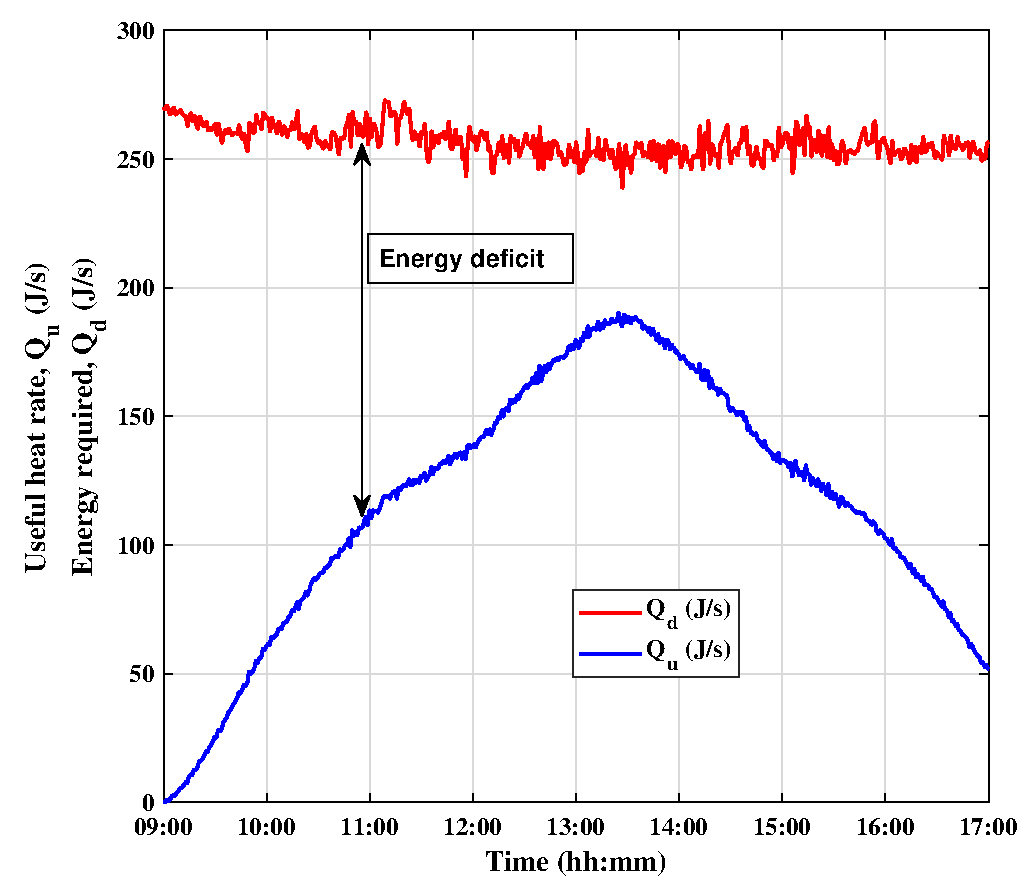
\includegraphics[scale=0.45]{figs/dry_low_1col.eps}
		\subcaption{Energy results at $\rm{m_{air}}$ = 26.10 kg/h.}
		
	\end{minipage}
	\begin{minipage}{0.50\columnwidth}
		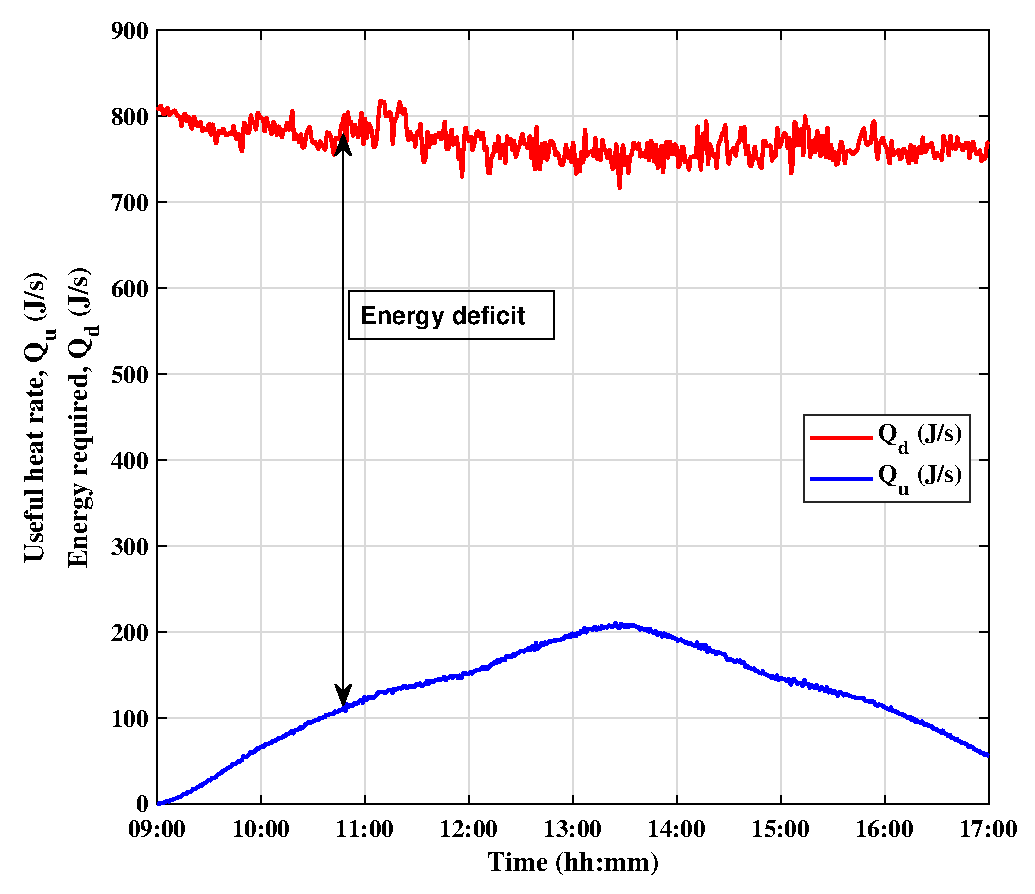
\includegraphics[scale=0.45]{figs/dry_high_1col.eps}
		\subcaption{Energy results at $\rm{m_{air}}$ = 78.30 kg/h.}
		
	\end{minipage}
	\caption{Simulated energies for two different airflow rates at the first collector in series.}
	\label{dry_1col}
\end{figure}

In Figure \ref{dry_1col}, which represents the energy at the output of the first solar collector, for both flow rates, there is an energy deficit between the supplied and required energy, necessitating the activation of the gas burner to bridge this gap. 

In Figure \ref{dry_2col}, illustrating the energy at the output of the second collector, for the lowest airflow rate, there is a period of operation (between 12:20 and 14:30) where the energy from the SAHS surpasses the required energy, resulting in a surplus, and thus, the burner does not need to operate. 

\begin{figure}[ht!]
	\begin{minipage}{0.50\columnwidth}
		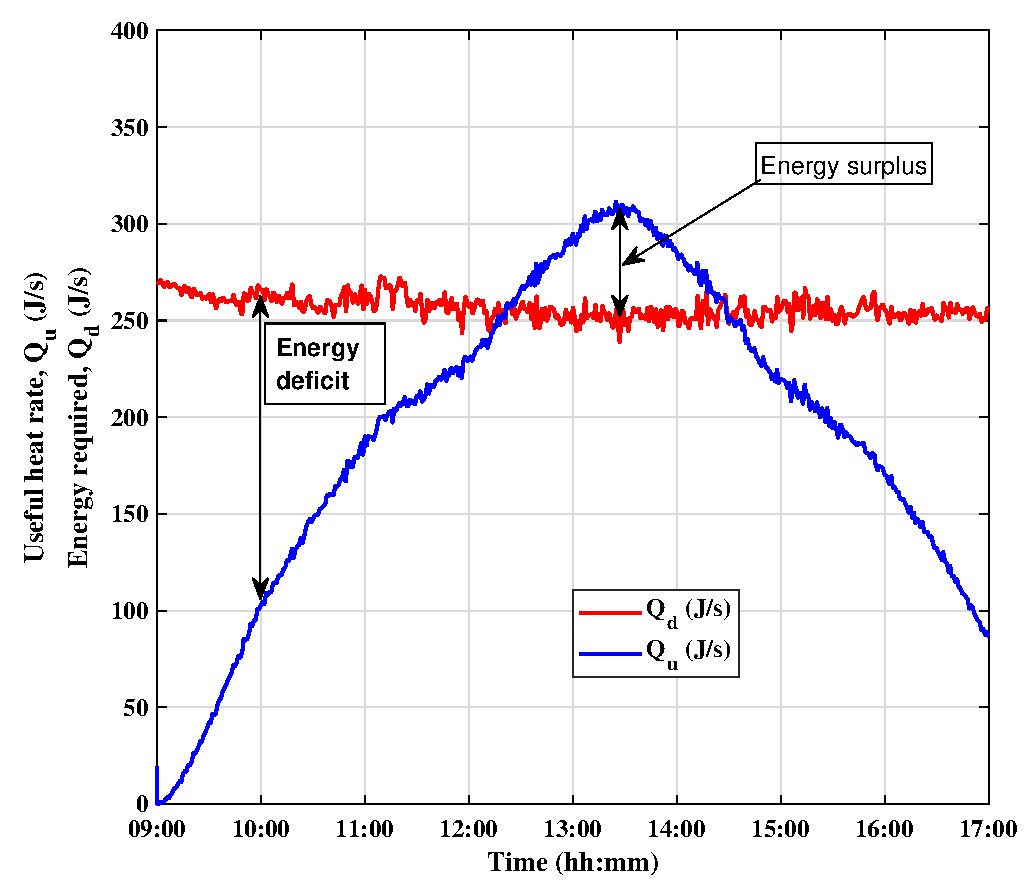
\includegraphics[scale=0.45]{figs/dry_low_2col.eps}
		\subcaption{Energy results at $\rm{m_{air}}$ = 26.10 kg/h.}
		
	\end{minipage}
	\begin{minipage}{0.50\columnwidth}
		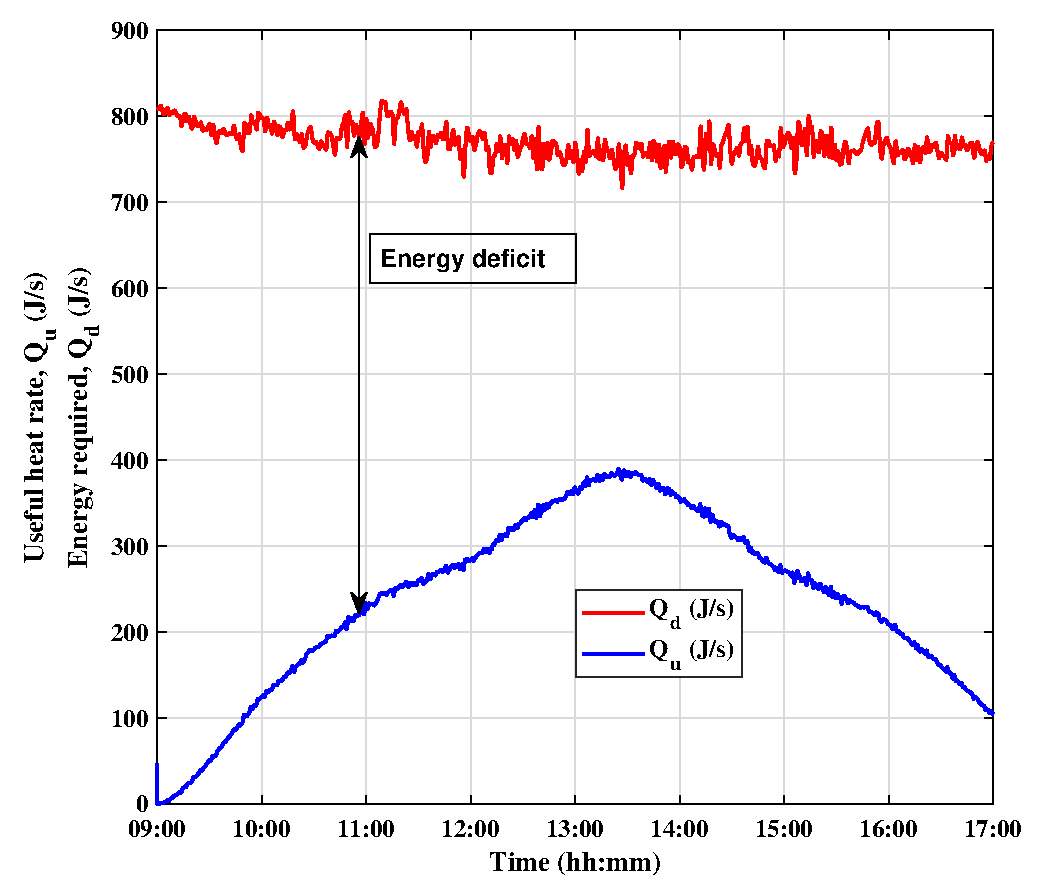
\includegraphics[scale=0.45]{figs/dry_high_2col.eps}
		\subcaption{Energy results at $\rm{m_{air}}$ = 78.30 kg/h.}
		
	\end{minipage}
	\caption{Simulated energies for two different airflow rates at the second collector in series.}
	\label{dry_2col}
\end{figure}

Figure \ref{dry_3col} shows that, at the output of the third collector, the period of surplus energy extends (between 11:30 and 15:00), requiring less from the burner. The energy deficit naturally decreases in the simulation with the highest airflow rate.

\begin{figure}[ht!]
	\begin{minipage}{0.50\columnwidth}
		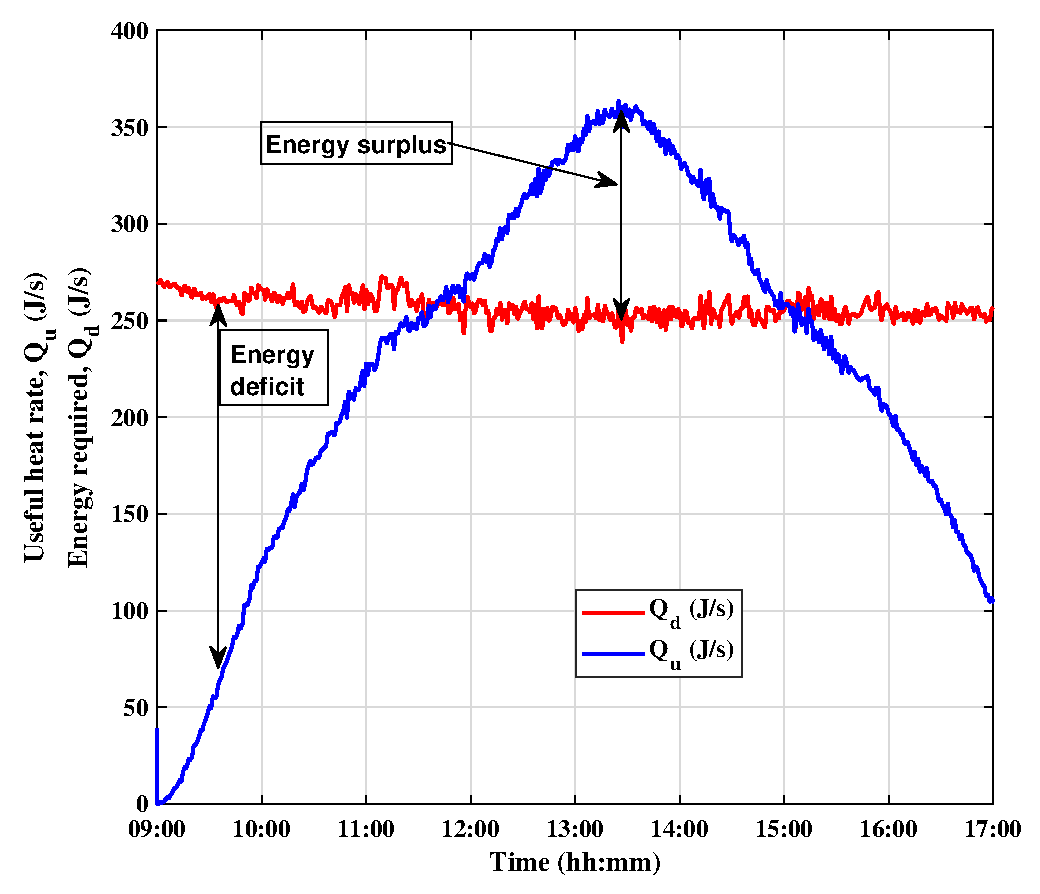
\includegraphics[scale=0.45]{figs/dry_low_3col.eps}
		\subcaption{Energy results at $\rm{m_{air}}$ = 26.10 kg/h.}
		
	\end{minipage}
	\begin{minipage}{0.50\columnwidth}
		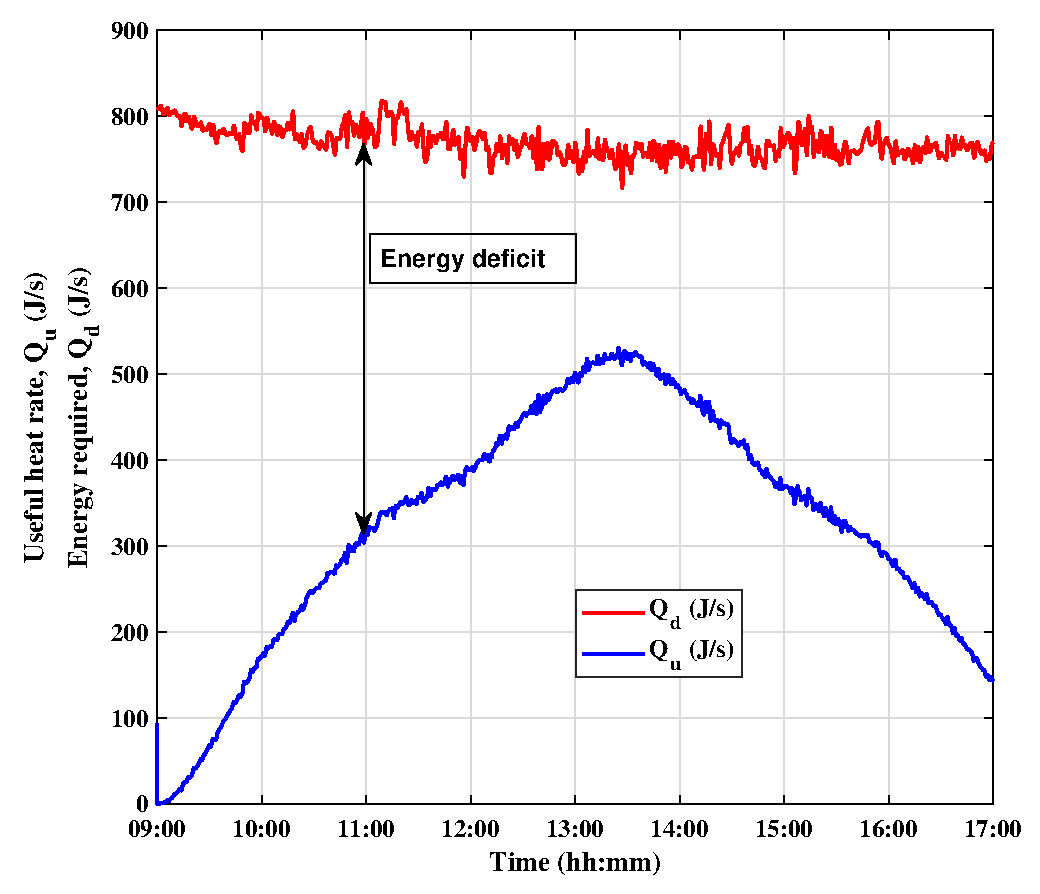
\includegraphics[scale=0.45]{figs/dry_high_3col.eps}
		\subcaption{Energy results at $\rm{m_{air}}$ = 78.30 kg/h.}
		
	\end{minipage}
	\caption{Simulated energies for two different airflow rates at the third collector in series.}
	\label{dry_3col}
\end{figure}

\subsection{Scenario 1 -- Air heating by gas burner alone}

The required heat rate transferred to the airflow by the gas burner is calculated by Eq. (\ref{usefulenergy}). Table \ref{gas-only} shows the values of energy required, mass dried, volume of natural gas burned and mass of $\rm{CO_2}$ released for each airflow level. At this airflow rate range and operating for 8 hours, 41 -- 122 kg of barley can be dried to reduce its moisture content from 20 to 15\% on a dry basis.

\begin{table}[h]
	\caption{Quantity of barley dried and amount of $\rm{CO_2}$ released for 8h of operation as function of the airflow rate only using gas burner for air heating.}
	\centering
	
	\begin{tabular}{ccccc}
		\hline \\ [-10pt]
		$\rm{m_{air}}$ (kg/h) & $\rm{Q_{req}}$ (kWh) & $\rm{M_{bar,dried}}$ (kg) & Gas volume (L) & $\rm{M_{CO2}}$ (kg) \\
		\hline \\ [-12pt]
		26.10 & 2.053 & 41 & 184.75 & 0.364 \\ [2pt]
		39.15 & 3.083 & 61 & 277.50 & 0.547 \\ [2pt]
		52.20 & 4.108 & 81 & 369.75 & 0.728 \\ [2pt]
		78.30 & 6.161 & 122 & 554.50 & 1.092 \\ 
		\hline
	\end{tabular}
	
	\label{gas-only}
\end{table}



\subsection{Scenario 2 -- Air heating using a gas burner and solar system}

In this scenario, the energy required to heat the airflow is partially provided by the SAHS and the complementary is by the gas burner. The connection of solar collectors in the system is considered. Table \ref{gas-solar} shows the values for a connection of up to 3 collectors in series of $\rm{Q_{req}}$ and $\rm{Q_u}$ by each mode, the volume of natural gas burned, the mass of $\rm{CO_2}$ released and the solar fraction for each airflow level. The solar fraction is the ratio of the energy the SAHS provides ($\rm{Q_u}$) and the energy required ($\rm{Q_{req}}$). Additionally, Table \ref{gas-solar-parallel} shows values for a connection of 3 collectors operating in parallel, where the total airflow rates are triple the values for the range in series (78.30 -- 235~kg/h).


\begin{table}[h]
	\caption{Quantity of barley dried and amount of $\rm{CO_2}$ released for 8 hours of operation as a function of the airflow rate using a gas burner and the solar system for air heating for connection of up to 3 collectors in series.}
	\centering
	
	\begin{tabular}{rrrrrrrr}
		\hline \\ [-10pt]
		 \makecell{$\rm{m_{air}}$ \\ (kg/h)} & \makecell{$\rm{Q_{req}}$ \\ (kWh)} & 	\makecell{$\rm{Q_{u}}$ \\ (kWh)} & 	\makecell{$\rm{Q_{burner}}$  \\ (kWh)} & \makecell{Gas Volume \\ (L)} & \makecell{$\rm{M_{CO2}}$  \\ (kg)} & \makecell{Solar \\ Fraction} \\
		\hline \\ [-10pt]
		\multicolumn{7}{c}{After the $\rm{1^{st}}$ collector} \\ \hline \\ [-10pt]
		26.10 & 2.053 & 0.933 & 1.119 & 100.75 & 0.198 & 0.4547 \\ [2pt]
		39.15 & 3.083 & 0.978 & 2.106 & 189.50 & 0.373 & 0.3171 \\ [2pt]
		52.20 & 4.108 & 1.000 & 3.108 & 279.75 & 0.551 & 0.2434 \\ [2pt]
		78.30 & 6.161 & 1.100 & 5.061 & 455.50 & 0.897 & 0.1785 \\
		\hline \\ [-10pt]
		\multicolumn{7}{c}{After the $\rm{2^{nd}}$ collector in series} \\ \hline \\ [-10pt]
		26.10 & 2.053 & 1.544 & 0.508 & 45.75 & 0.090 & 0.7524 \\ [2pt]
		39.15 & 3.083 & 1.635 & 1.448 & 130.31 & 0.257 & 0.5304 \\ [2pt]
		52.20 & 4.108 & 1.726 & 2.382 & 214.38 & 0.422 & 0.4202 \\ [2pt]
		78.30 & 6.161 & 1.908 & 4.253 & 382.75 & 0.754 & 0.3097 \\ 
		\hline \\ [-10pt]
		\multicolumn{7}{c}{After the $\rm{3^{rd}}$ collector in series} \\ \hline \\ [-10pt]
		26.10 & 2.053 & 1.819 & 0.233 & 21.00 & 0.041 & 0.7904 \\ [2pt]
		39.15 & 3.083 & 2.015 & 1.068 & 96.13 & 0.189 & 0.6850 \\ [2pt]
		52.20 & 4.108 & 2.211 & 1.897 & 170.75 & 0.336 & 0.5766 \\ [2pt]
		78.30 & 6.161 & 2.603 & 3.558 & 320.25 & 0.631 & 0.4225 \\
		\hline
	\end{tabular}
	
	\label{gas-solar}
\end{table}

The amount of barley dried is the same as in Table \ref{gas-only} as the air temperature is set to 60 $^{\rm{o}}$C to enter the dryer. For 3 collectors in series, the SAHS can offset from 42 to 79\% of the energy the gas burner provided alone. 

\begin{table}[h]
	\caption{Quantity of barley dried and amount of $\rm{CO_2}$ released for 8h of operation as a function of the airflow rate using a gas burner and sothe lar system for air heating for connection of 3 collectors in parallel.}
	\centering
	
	\begin{tabular}{rrrrrrrr}
		\hline \\ [-10pt]
		\makecell{$\rm{m_{air}}$ \\ (kg/h)} & \makecell{$\rm{Q_{req}}$ \\ (kWh)} & 	\makecell{$\rm{Q_{u}}$ \\ (kWh)} & 	\makecell{$\rm{Q_{burner}}$  \\ (kWh)} & \makecell{Gas Volume \\ (L)} & \makecell{$\rm{M_{CO2}}$  \\ (kg)} & \makecell{Solar \\ Fraction} \\
		\hline \\ [-10pt]
		3x26.10 & 6.161 & 4.870 & 1.291 & 116.20 & 0.229 & 0.7904 \\ [2pt]
		3x39.15 & 9.250 & 6.336 & 2.914 & 262.55 & 0.517 & 0.6850 \\ [2pt]
		3x52.20 & 12.325 & 7.107 & 5.218 & 469.66 & 0.925 & 0.5766 \\ [2pt]
		3x78.30 & 18.483 & 7.810 & 10.673 & 960.60 & 1.892 & 0.4225 \\ 
		\hline
	\end{tabular}
	
	\label{gas-solar-parallel}
\end{table}

\newpage
Considering collectors operating in parallel, the energy required is increased due to higher airflow levels. The useful energy collected by the solar system is also higher. The solar fraction calculated is the same as obtained when the system is operated in series, meaning that both connections will offset the same energy levels relative to the required ones. The advantage of operating in parallel over in series is that the amount of barley dried is increased by 3 times: 122 -- 366 kg of barley can be dried to reduce its moisture content from 20 to 15\% on a dry basis.




\subsection{Scenario 3 -- Air heating using the solar system alone}

In this scenario, the SAHS alone provides energy to the airflow. Most of the time, the solar energy is insufficient to rise the temperature to 60~$^{\rm{o}}$C, resulting in low drying rates and, therefore, in a lower dried mass of barley. Table \ref{solar-only} shows the mass of barley that can be dried if only the SAHS is used in the operation. The quantity of mass dried varies from 22 -- 61 kg, notably less than other systems as the drying rate is lower. 

\begin{table}[h]
	\caption{Quantity of barley dried and amount of $\rm{CO_2}$ released for 8h of operation as a function of the airflow rate using the solar system alone for air heating for connection of 3 collectors in series.}
	\centering
	
	\begin{tabular}{cccccccc}
		\hline \\ [-10pt]
		\multirow{2}{*}{ $\rm{m_{air}}$  (kg/h)} & \multicolumn{2}{c}{After $\rm{1^{st}}$ collector} & \multicolumn{2}{c}{After $\rm{2^{nd}}$ collector} & \multicolumn{2}{c}{After $\rm{3^{rd}}$ collector} \\
		
		 & \makecell{$\rm{Q_{u}}$ \\ (kWh)} & 	\makecell{$\rm{M_{bar,dried}}$ \\ (kg)} & 	\makecell{$\rm{Q_{u}}$  \\ (kWh)} & \makecell{$\rm{M_{bar,dried}}$ \\ (kg)} & \makecell{$\rm{Q_{u}}$  \\ (kWh)} & \makecell{$\rm{M_{bar,dried}}$ \\ (kg)} \\
		\hline \\ [-10pt]
		26.10 & 0.933 & 22 & 1.544 & 33 & 1.819 & 37 \\ [2pt]
		39.15 & 0.978 & 24 & 1.635 & 37 & 2.015 & 43 \\ [2pt]
		52.20 & 1.000 & 25 & 1.726 & 40 & 2.211 & 50 \\ [2pt]
		78.30 & 1.100 & 28 & 1.908 & 47 & 2.603 & 61 \\ 
		\hline
	\end{tabular}
	
	\label{solar-only}
\end{table}

When the air heating collectors are connected in parallel, the thermal energy absorbed by the airflow rate is higher, which results in more mass dried, as shown in Table \ref{gas-only-parallel}. As the airflow rate tripled, the quantity of barley dried also tripled (66 -- 84 kg), which is an advantage over the connection in series.

\begin{table}[h]
	\caption{Quantity of barley dried and amount of $\rm{CO_2}$ released for 8h of operation as a function of the airflow rate using the solar system alone for air heating for connection of 3 collectors in parallel.}
	\centering
	
	\begin{tabular}{ccc}
		\hline \\ [-10pt]
		$\rm{m_{air}}$ (kg/h) & $\rm{Q_{u}}$ (kWh) & $\rm{M_{bar,dried}}$ (kg) \\
		\hline \\ [-10pt]
		3x26.10 & 2.800 & 66 \\ [2pt]
		3x39.15 & 2.933 & 72 \\ [2pt]
		3x52.20 & 3.000 & 75 \\ [2pt]
		3x78.30 & 3.300 & 84 \\ 
		\hline
	\end{tabular}
	
	\label{gas-only-parallel}
\end{table}

%From the airflow range used in this research, one common level can be taken to compare the 3 scenarios treated previously, which is 78.3 kg/h. This comparison can be made considering mass of barley dried, volume of natural gas burnt and solar fraction, as shown in Table \ref{scenario-comparison}.  The data suggests that the use of solar air heating systems can significantly reduce the reliance on gas heating, with the gas burner + SAHS in parallel system having the lowest consumption of gas and highest solar fraction of all the systems listed. However, the choice of heating system will depend on various factors, including the availability of sunlight, the cost and availability of natural gas.

In this study, a particular airflow range was utilized, and a common level of 78.3~kg/h can be used to compare the three previously analyzed scenarios. This assessment can be conducted by examining the mass of dried barley, the amount of natural gas burned, and the solar fraction, all presented in Table \ref{scenario-comparison}.  The gas burner system has the highest gas volume consumption of 554.5 L and a solar fraction of 0, meaning it relies completely on gas for heating. On the other hand, the SAHS standalone system produces less dried mass, but both connections have a solar fraction of 1, indicating that they rely solely on solar energy. The results indicate that the SAHS can substantially reduce dependence on natural gas heating. Specifically, the gas burner + SAHS in parallel configuration exhibited the lowest gas consumption and highest solar fraction among all the listed systems with a gas burner. Nevertheless, selecting a heating system will depend on factors such as sunlight availability, natural gas cost, and accessibility.

\begin{table}[h]
	\caption{Comparison of the 3 scenarios at $\rm{m_{air}}$ = 78.3 kg/h for 8h of operation. }
	\centering
	
	\begin{tabular}{lrrr}
		\hline \\ [-10pt]
		Type of system & $\rm{M_{bar,dried}}$ (kg) & Gas volume (L) & Solar fraction \\
		\hline \\ [-10pt]
		Gas burner only & 122 & 554.50 & 0.00 \\ [2pt]
		Gas burner + SAHS series & 122 & 320.25 & 0.42 \\ [2pt]
		Gas burner + SAHS parallel & 122 & 116.20 & 0.79 \\ [2pt]
		SAHS series & 61 & 0.00 & 1.00 \\ [2pt] 
		SAHS parallel & 65 & 0.00 & 1.00 \\
		\hline
	\end{tabular}
	
	\label{scenario-comparison}
\end{table}

\section{Chapter Summary}

Thermal modelling and simulation of the proposed solar air heating system were developed and validated against experimental data. Results show that, in general, the heat transfer model underestimates 65\% of the data, and 95\% of the residues generated are between $\pm$2 $^{\rm{o}}$C and $\pm$50 W/m$^2$. Overall, the mean absolute error in temperature was 2\%, and useful energy was 8\%. After validation, the system has been characterised within a certain range of inputs.

The model was also used to simulate results at nearly steady-state conditions. The thermal efficiency curve was plotted and compared to the experimental one. The parameters of the Hottel-Whillier-Bliss equation $\rm{F_{\!_R}}\eta_{\rm{o}}$ and $\rm{ F_{\!_R}{U_{\!_L}}}$ calculated by the thermal model are 0.64 and -3.02, with relative differences of 2\% and 10\%, respectively, in relation to the parameters of the experimental data.

Thermal modelling was also used to predict the thermal performance of three connected collectors in series and parallel. The connection in series can deliver higher outlet airflow temperatures. In contrast, the connection in parallel can collect more useful heat but deliver the same airflow temperature as if it is leaving the first collector in series.

Lastly, this model was used to simulate barley drying. Three scenarios were considered to meet the energy demand: simulating only a gas burner to heat the airflow to 60 $^{\rm{o}}$C; simulating the SAHS and a gas burner to heat the airflow to 60 $^{\rm{o}}$C, and; simulating only the SAHS to heat the airflow with no air temperature limit. From a specific airflow level , the gas burner system has the highest gas volume consumption and a solar fraction of 0, meaning it relies completely on gas for heating. On the other hand, the SAHS standalone system produces less dried mass, but both connections have a solar fraction of 1, indicating that they rely solely on solar energy. The results indicate that using SAHS can substantially reduce dependence on natural gas heating. Specifically, the gas burner + SAHS in parallel configuration exhibited the lowest gas consumption and highest solar fraction among all the listed systems with a gas burner. Nevertheless, the selection of a heating system will depend on various factors, such as sunlight availability, natural gas cost, and accessibility.


%A for abbreviations
\nomenclature[A]{ODE}{Ordinary Differential Equation}
\nomenclature[A]{CPC}{Compound Parabolic Concentrator}
\nomenclature[A]{ACPC}{Asymmetric Compound Parabolic Concentrator}
\nomenclature[A]{CFD}{Computational Fluid Dynamics}
\nomenclature[A]{IACPC}{Inverted Absorber Compound Parabolic Concentrator}
\nomenclature[A]{SAHS}{Solar Air Heating System}
\nomenclature[A]{ESTTP}{European Solar Thermal Technology Platform}
\nomenclature[A]{SAHC}{Solar Air Heating Collector}
\nomenclature[A]{GAHC}{Glazed Air Heating Collector}
\nomenclature[A]{PTC}{Parabolic Trough Concentrator}
\nomenclature[A]{UTSC}{Unglazed Transpired Solar Collector}
\nomenclature[A]{BISTS}{Building Integrated Solar Thermal System}


%N for latin
\nomenclature[N]{$\rm{r_{par}}$}{Parallel component of unpolarized radiation}
\nomenclature[N]{$\rm{r_{perp}}$}{Perpendicular component of unpolarized radiation}
\nomenclature[N]{$\rm{n_{idx}}$}{Glazing's refractive index}
\nomenclature[N]{$\rm{K_{ext}}$}{Glazing's extinction coefficient [m$^{-1}$]}
\nomenclature[N]{$\rm{N_{c}}$}{Number of glazing covers}
\nomenclature[N]{$\rm{r_{inc}}$}{Vector of the incident ray}
\nomenclature[N]{$\rm{r_{ref}}$}{Vector of the reflected ray}
\nomenclature[N]{$\rm{r_{n}}$}{Vector normal at the intersect point}
\nomenclature[N]{$\rm{m_{air}}$}{Mass airflow rate [kg/h]}
\nomenclature[N]{$\rm{u_{g}}$}{Systematic uncertainty related to the airflow rate [kg/(s.m$^2$)]}
\nomenclature[N]{$\rm{V_{a}}$}{Voltage input supplied by the adaptor [V]}
\nomenclature[N]{$\rm{F_{R}}$}{Heat removal factor}
\nomenclature[N]{$\rm{U}$}{Internal energy [J]}
\nomenclature[N]{$\rm{S}$}{Solar radiation rate absorbed [W]}
\nomenclature[N]{$\rm{Q_{u}}$}{Useful energy rate transferred to the airflow [W or J/s]}
\nomenclature[N]{$\rm{Q_{req}}$}{Energy required to heat the airflow to 60 \textdegree C [W or J/s]}
\nomenclature[N]{$\rm{Q_{dryer}}$}{Energy demand to dried a certain mass of barley [W or J/s]}
\nomenclature[N]{$\rm{Q_{burner}}$}{Energy provided by the gas burner [W or J/s]}
\nomenclature[N]{$\rm{t}$}{Time [s]}
\nomenclature[N]{$\rm{R}$}{Thermal resistance [\textdegree C/W]}
\nomenclature[N]{$\rm{h}$}{Heat transfer coefficient [W/(m$^2$.\textdegree C)]}
\nomenclature[N]{$\rm{T}$}{Temperature [\textdegree C]}
\nomenclature[N]{$\rm{M}$}{Mass [kg]}
\nomenclature[N]{$\rm{I_D}$}{Diffuse solar radiation [W/m$^2$]}
\nomenclature[N]{$\rm{I_B}$}{Beam solar radiation [W/m$^2$]}
\nomenclature[N]{$\rm{CR}$}{Geometric concentration ratio}
\nomenclature[N]{$\rm{I_T}$}{Global solar radiation [W/m$^2$]}
\nomenclature[N]{$\rm{A}$}{Area [m$^2$]}
\nomenclature[N]{$\rm{L_{col}}$}{Collector length [m]}
\nomenclature[N]{$\rm{Re}$}{Reynolds number}
\nomenclature[N]{$\rm{Ra}$}{Rayleigh number}
\nomenclature[N]{$\rm{Pr}$}{Prandtl number}
\nomenclature[N]{$\rm{W}$}{Width [m]}
\nomenclature[N]{$\rm{k_{air}}$}{Air thermal conductivity [W/(m.\textdegree C)]}
\nomenclature[N]{$\rm{C_{p}}$}{Specific heat [J/(kg.\textdegree C)]}
\nomenclature[N]{$\rm{G_{air}}$}{Mass airflow rate based on the absorber area [kg/(s.m$^2$)]}
\nomenclature[N]{$\rm{A_{abs}^{'}}$}{Absorber area without the holes [m$^2$]}
\nomenclature[N]{$\rm{Nu}$}{Nusselt number}
\nomenclature[N]{$\rm{v}$}{Air velocity [m/s]}
\nomenclature[N]{$\rm{g}$}{Acceleration due to gravity [9.81 m/s$^2$]}
\nomenclature[N]{$\rm{H}$}{Height [m]}
\nomenclature[N]{$\rm{U_L}$}{Overall heat loss coefficient [W/(m$^2$.\textdegree C)]}
\nomenclature[N]{$\rm{d_{air}}$}{Air density [kg/m$^3$]}
\nomenclature[N]{$\rm{N_{obs}}$}{Number of observations}
\nomenclature[N]{$\rm{Y_{exp}}$}{Experimental or observed value of the variable Y}
\nomenclature[N]{$\rm{Y_{sim}}$}{Simulated of predicted value of the variable Y}
\nomenclature[N]{$\rm{a_{s}}$}{Altitude solar angle [degrees]}
\nomenclature[N]{$\rm{t_{ST}}$}{Solar time [h]}
\nomenclature[N]{$\rm{t_{LST}}$}{Local standard time [h]}
\nomenclature[N]{$\rm{E_{T}}$}{Equation of time [min]}
\nomenclature[N]{$\rm{f}$}{Focal distance [m]}
\nomenclature[N]{$\rm{X_{in}}$}{Barley moisture content at the dryer's inlet (in dry base)}
\nomenclature[N]{$\rm{X_{out}}$}{Barley moisture content at the dryer's outlet (in dry base)}
\nomenclature[N]{$\rm{x}$}{x-coordinates}
\nomenclature[N]{$\rm{y}$}{y-coordinates}
\nomenclature[N]{$\rm{z}$}{z-coordinates}
\nomenclature[N]{$\rm{t_{p}}$}{Parametric variable in the xy-plane}
\nomenclature[N]{$\rm{{\overline W}_{glaz}}$}{Glazing characteristic length [m]}
\nomenclature[N]{$\rm{W_{col}}$}{Collector depth [m]}
\nomenclature[N]{$\rm{y_{TS}}$}{y-coordinate of the tertiary section position}
\nomenclature[N]{$\rm{x_{apt}}$}{x-coordinate of the aperture position}
\nomenclature[N]{$\rm{y_{apt,upper}}$}{y-coordinate of the aperture at the upper parabola}
\nomenclature[N]{$\rm{y_{apt,lowper}}$}{y-coordinate of the aperture at the lower parabola}

%P for greek
\nomenclature[P]{$\Gamma$}{Intercept factor}
\nomenclature[P]{$\rm{\ell}$}{Hole pitch [m]}
\nomenclature[P]{$\rm{\varphi_p}$}{Absorber porosity}
\nomenclature[P]{$\rm{\varphi_h}$}{Hole size [m]}
\nomenclature[P]{$\Delta \rm{t}$}{Time step [s]}
\nomenclature[P]{$\nu_{\rm{air}}$}{Air kinematic viscosity [m$^2$/s]}
\nomenclature[P]{$\varepsilon_{\rm{eff}}$}{Effective emissivity}
\nomenclature[P]{$\varepsilon$}{Infrared emissivity}
\nomenclature[P]{$\alpha$}{Absorptivity}
\nomenclature[P]{$\sigma$}{Stefan-Boltzmann constant [$5.67$ \rm{x} ${10^{-8}}$ W/(m$^2$.K$^4$)]}
\nomenclature[P]{$\eta_{\rm{th}}$}{Thermal efficiency}
\nomenclature[P]{$\eta_{\rm{o}}$}{Optical efficiency}
\nomenclature[P]{$\xi$}{Mean absolute error}
\nomenclature[P]{$\tau$}{Transmissivity}
\nomenclature[P]{$\gamma_{\rm{col}}$}{Collector's azimuth angle [degrees]}
\nomenclature[P]{$\gamma_{\rm{s}}$}{Solar azimuth angle [degrees]}
\nomenclature[P]{$\tau_{\rm{col}}$}{Collector's transmissivity}
\nomenclature[P]{$\delta$}{Thickness [m]}
\nomenclature[P]{$\theta_{\rm{i}}$}{Incident angle at the glazing cover [degrees]}
\nomenclature[P]{$\theta_{\rm{r}}$}{Refracted angle in the glazing cover [degrees]}
\nomenclature[P]{$\rho$}{Reflectivity}
\nomenclature[P]{$\theta_{\rm{P1}}$}{Angle of the upper parabola axis to the horizontal [degrees]}
\nomenclature[P]{$\theta_{\rm{P2}}$}{Angle of the lower parabola axis to the horizontal [degrees]}
\nomenclature[P]{$\theta_{\rm{acc}}$}{Angular acceptance for a specific parabola [degrees]}
\nomenclature[P]{$\theta_{\rm{a}}$}{Angular parameter for a specific parabola [degrees]}
\nomenclature[P]{$\rm{\ell_{ST}}$}{Standard longitude angle [degrees]}
\nomenclature[P]{$\rm{\ell_{local}}$}{Local longitude angle [degrees]}
\nomenclature[P]{$\omega_{\rm{s}}$}{Solar hour angle [degrees]}
\nomenclature[P]{$\delta_{\rm{s}}$}{Solar declination angle [degrees]}
\nomenclature[P]{$\phi$}{Local latitude angle [degrees]}
\nomenclature[P]{$\beta$}{Glazing inclination angle [degrees]}
\nomenclature[P]{$\Delta{\rm{x}}$}{Displacement of the parabola in the x-coordinates [m]}
\nomenclature[P]{$\Delta{\rm{y}}$}{Displacement of the parabola in the y-coordinates [m]}
\nomenclature[P]{$\theta_{\rm{iy}}$}{Angle of the solar ray to the horizontal in the xy-plane [degrees]}
\nomenclature[P]{$\theta_{\rm{iz}}$}{Angle of the solar ray to the horizontal in the xz-plane [degrees]}
\nomenclature[P]{$\lambda_{\rm{v}}$}{Latent heat of vaporisation [J/kg]}

%S for subscripts
\nomenclature[S]{in}{Inlet}
\nomenclature[S]{out}{Outlet}
\nomenclature[S]{h}{Hole}
\nomenclature[S]{w}{Wind}
\nomenclature[S]{R1}{Radiation from absorber to glazing}
\nomenclature[S]{C1}{Convection from absorber to glazing}
\nomenclature[S]{R2}{Radiation from glazing to ambient}
\nomenclature[S]{C2}{Convection from glazing to ambient}
\nomenclature[S]{HX}{Convection from absorber to airflow}
\nomenclature[S]{abs}{Absorber plate}
\nomenclature[S]{glaz}{Glazing cover}
\nomenclature[S]{amb}{Ambient}
\nomenclature[S]{apt}{Aperture}
\nomenclature[S]{TS}{Tertiary section}
\nomenclature[S]{avg}{Average}
\nomenclature[S]{v}{Vaporization point}
\nomenclature[S]{bar}{Barley grains}
\nomenclature[S]{col}{Collector}
\nomenclature[S]{ref}{Reflector}
\nomenclature[S]{int}{Intersection point}
\nomenclature[S]{wl}{Liquid water}



